\documentclass[draft, final]{vutinfth} % Remove option 'final' to obtain debug information.

\usepackage{ifxetex}
\ifxetex
    \usepackage{fontspec}
    \defaultfontfeatures{Mapping=tex-text}
    
    %\setsansfont{Fira Sans}
    %\setsansfont{Lato}
    %\setsansfont{Roboto}
    \setsansfont{Source Sans Pro}

    %\setmainfont{Noto Serif}
    \setmainfont{Source Serif Pro}
    
    %\setmonofont{Fira Code}
    \setmonofont{Source Code Pro}
\else
    % Load packages to allow in- and output of non-ASCII characters.
    \usepackage{lmodern}        % Use an extension of the original Computer Modern font to minimize the use of bitmapped letters.
    \usepackage[T1]{fontenc}    % Determines font encoding of the output. Font packages have to be included before this line.
    \usepackage[utf8]{inputenc} % Determines encoding of the input. All input files have to use UTF8 encoding.
\fi

% Extended LaTeX functionality is enables by including packages with \usepackage{...}.
\usepackage{fancyvrb}
\usepackage{listings}
\usepackage{amsmath}    % Extended typesetting of mathematical expression.
\usepackage{amssymb}    % Provides a multitude of mathematical symbols.
\usepackage{mathtools}  % Further extensions of mathematical typesetting.
\usepackage{microtype}  % Small-scale typographic enhancements.
\usepackage[inline]{enumitem} % User control over the layout of lists (itemize, enumerate, description).
\usepackage{multirow}   % Allows table elements to span several rows.
\usepackage{booktabs}   % Improves the typesetting of tables.
\usepackage{subcaption} % Allows the use of subfigures and enables their referencing.
\usepackage[ruled,linesnumbered,algochapter]{algorithm2e} % Enables the writing of pseudo code.
\usepackage[usenames,dvipsnames,table]{xcolor} % Allows the definition and use of colors. This package has to be included before tikz.
\usepackage{nag}       % Issues warnings when best practices in writing LaTeX documents are violated.
\usepackage{todonotes} % Provides tooltip-like todo notes.
\usepackage{hyperref}  % Enables hyperlinking in the electronic document version. This package has to be included second to last.
\usepackage[acronym,toc]{glossaries} % Enables the generation of glossaries and lists of acronyms. This package has to be included last.

\uselanguage{english}
%\renewcommand{\familydefault}{\sfdefault}

%\bibstyle{plain}
%\bibdata{main}

% Define convenience functions to use the author name and the thesis title in the PDF document properties.

% Set PDF document properties
\hypersetup{
    pdfpagelayout   = SinglePage,           % How the document is shown in PDF viewers (optional).
    linkbordercolor = {Blue},                 % The color of the borders of boxes around crosslinks (optional).
    pdfauthor       = {\authorname},          % The author's name in the document properties (optional).
    pdftitle        = {\thesistitle},         % The document's title in the document properties (optional).
    pdfsubject      = {Subject},              % The document's subject in the document properties (optional).
    pdfkeywords     = {Photovoltaik, study, VR} % The document's keywords in the document properties (optional).
}

\setpnumwidth{2.5em}        % Avoid overfull hboxes in the table of contents (see memoir manual).
\setsecnumdepth{subsection} % Enumerate subsections.
\nonzeroparskip             % Create space between paragraphs (optional).
\setlength{\parindent}{0pt} % Remove paragraph identation (optional).
% \setlist[itemize]{itemsep=0pt, topsep=0pt, parsep=0pt, partopsep=0pt}
% \OnehalfSpacing
% \sloppy
\hyphenpenalty=800
\tolerance=2000
\emergencystretch=3em

\fvset{
  fontsize=\fontsize{8pt}{10pt}
}
\lstset{basicstyle=\ttfamily\small}

\makeindex      % Use an optional index.
% \makeglossaries % Use an optional glossary.
%\glstocfalse   % Remove the glossaries from the table of contents.

% Set persons with 4 arguments:
% {title before name}{name}{title after name}{gender}
% where both titles are optional (i.e. can be given as empty brackets {}).
% For bachelor and master theses:
% \setfirstassistant{Pretitle}{Forename Surname}{Posttitle}{male}
% \setsecondassistant{Pretitle}{Forename Surname}{Posttitle}{male}
% \setthirdassistant{Pretitle}{Forename Surname}{Posttitle}{male}

\setdate{31}{8}{2024} % Set date with 3 arguments: {day}{month}{year}.
\newcommand{\authorname}{Daniel Jonas Otto} % The author name without titles.
\setauthor{}{\authorname}{}{male}
\setregnumber{11811332}

\setadvisor{Dipl.-Ing.in Dr.in}{Katharina Krösl}{}{female}

 % The title of the thesis. The English version should be used, if it exists.
\newcommand{\thesistitle}{Empowering the Energy Transition Through Virtual Reality}
\settitle{\thesistitle}{}{}
\setsubtitle{A Case Study on Promoting Photovoltaic Solutions}{}
\setthesis{bachelor}
\setcurriculum{Software and Information Engineering}{Software und Information Engineering}

\begin{document}

\frontmatter % Switches to roman numbering.
% The structure of the thesis has to conform to the guidelines at
%  https://informatics.tuwien.ac.at/study-services

\addtitlepage{english} % English title page.
\addstatementpage

\begin{acknowledgements*}
I want to express my heartfelt gratitude to everyone who supported me throughout the creation of this thesis. 

My deepest thanks go to my partner, Astrid Gaderbauer, for her unwavering patience, understanding, and encouragement during this demanding process. Her support was invaluable in helping me navigate the challenges and stay focused on my goals.

I am incredibly grateful to my advisor, Katharina Krösl, for her exceptional guidance, expertise, and unwavering support throughout this project. Her insightful feedback, constructive criticism, and encouragement were instrumental in shaping my research and pushing me to achieve my full potential.

I would also like to extend my sincere thanks to Helwin Prohaska from Energiewende Linz for his invaluable guidance and support in the development of the VR application. His expertise in the field of renewable energy and his passion for promoting sustainable solutions were truly inspiring.

A huge thank you to Sandro and Lukas from Energiewende Linz for their fantastic help in building the simulation in Unreal Engine. Their expertise in simulation and game development was crucial in ensuring the accuracy and effectiveness of the VR application.

Furthermore, I would like to express my gratitude to my grandparents for their generous financial support, which allowed me to devote myself to this research. Their belief in my vision and their encouragement throughout this journey were deeply appreciated.

Finally, I want to thank all the participants who took part in the user studies. Their valuable feedback and insights were essential in shaping the development and evaluation of \textit{SolarPowerVR}.

%I would like to express my gratitude to all those who have provided me with support in the creation of this work. In particular, I would like to thank my partner, Astrid Gaderbauer, for her assistance and understanding throughout this process. I would also like to acknowledge Helwin Prohaska for his invaluable guidance and support in the development of the VR application. Furthermore, I would like to extend my gratitude to my grandparents for their financial support and encouragement. Finally, I would like to express my gratitude to my supervisor, Katharina Krösl, for her extensive guidance and feedback throughout the entirety of this project.

% sandro for helping with the sun simulation formulas
% lukas for the help with implementing the sun calculation in unreal blueprints
\end{acknowledgements*}

% \begin{kurzfassung}
% \the\baselineskip
% % print fontsize
% \the\fontdimen6\font
% \end{kurzfassung}

\begin{abstract}
This thesis investigates the potential of Virtual Reality (VR) as a catalyst for promoting the energy transition in Austria, specifically focusing on increasing understanding and adoption of photovoltaic (PV) systems. Addressing the prevailing perception of the energy transition as complex and unattainable, this research leverages VR's immersive capabilities to demonstrate the feasibility and benefits of transitioning to renewable energy sources.

We first evaluate \textit{KaisergasseVR}, an existing VR application showcasing climate-friendly solutions in an urban context, to establish a baseline understanding of user experience and learning outcomes. Building upon this, we develop \textit{SolarPowerVR}, a novel VR application designed to provide an interactive and engaging learning experience focused on PV systems. \textit{SolarPowerVR} allows users to explore a realistic virtual environment, manipulate PV panel configurations, and observe the resulting impact on energy production under varying conditions, fostering a deeper understanding of PV system dynamics.

Our findings reveal that \textit{SolarPowerVR} significantly enhances user understanding of PV systems compared to \textit{KaisergasseVR}, highlighting the importance of interactive engagement in VR-based learning. However, the results also indicate that interactivity alone may not be sufficient for acquiring specific factual knowledge, such as optimal panel orientation. We discuss these findings in the context of existing research on VR in education and climate change communication, emphasizing the need for careful design choices that balance interactivity with clear instruction and guidance.

This thesis contributes to the growing body of knowledge on the potential of VR for environmental education and advocacy. By demonstrating the effectiveness of \textit{SolarPowerVR} in enhancing understanding of PV systems, we provide valuable insights for the design of future VR educational tools aimed at promoting sustainable energy solutions and contributing to a more sustainable future.
\end{abstract}

\tableofcontents % Starred version, i.e., \tableofcontents*, removes the self-entry.
\mainmatter

\chapter{Introduction}

The need to transition from fossil fuels to renewable energy sources has become a pressing global concern. The alarming pace of climate change, largely driven by our continued reliance on unsustainable energy practices, demands immediate action \cite{IPCC_2018_SR15}. In this context, photovoltaic (PV) systems, which utilize the abundant and clean energy of the sun, are a promising solution. However, despite the many benefits of PV technology, significant challenges remain, and overcoming these hurdles is critical to ensuring a sustainable energy future \cite{iea2020world}.

Austria, with its existing hydropower resources, has the potential to play a leading role in this transition. The European Climate Law, which legally binds all member states to achieve climate neutrality by 2050, underscores the urgency of action \cite{EUClimateLaw}.
While Austria has achieved a commendable 72\% share of renewable electricity, only 33\% of the country's total energy consumption comes from renewable sources. Emissions from industry, especially steel production, remain high and rising (25 Mt CO2eq). The transport sector, the second largest contributor to Austria's carbon footprint (21 Mt CO2eq), remains heavily dependent on oil. Austria's total gas consumption has increased by 30\% since 1990 \cite{StatistikAustria2024Energiebilanzen}. Meeting the EU targets will require a dramatic acceleration in the deployment of renewable energy solutions. This will require effective policy adjustments, streamlined implementation strategies, and a fundamental shift in public perception and acceptance of sustainable solutions.

However, effectively communicating the benefits and encouraging the adoption of technologies such as photovoltaic (PV) systems requires innovative approaches that go beyond traditional methods such as brochures and websites. While valuable, these methods often struggle to provide the level of engagement and experiential learning needed to inspire widespread behavior change \cite{Hassan2020Digitality}. This thesis explores the potential of virtual reality (VR) as such an innovative tool for environmental education, specifically focusing on increasing awareness and understanding of PV systems to catalyze their adoption in Austria. Despite the growing body of research highlighting the potential of VR in education \cite{HuAu2018VrExperience,Merchant2014VrEffectiveness} and promoting pro-environmental behaviors \cite{Queiroz2023Efficacy,McEvoy2023Climate}, a critical gap remains in its application to public education about PV technology. Existing resources often lack the engaging and immersive qualities of VR, particularly in providing experiences that foster a sense of ownership over energy choices. VR can fill this gap by offering unique advantages, including the ability to create immersive and interactive learning environments that can enhance understanding \cite{HuAu2018VrExperience, Winn2002Immersion}, promote spatial reasoning \cite{Dalgarno2010Learning, Sung2015Effects, Winn2002Immersion}, and foster a sense of agency and empowerment \cite{Gee2009Deep}. By allowing users to directly manipulate and experiment with PV systems in a safe and controlled virtual environment, VR can facilitate a deeper understanding of the technology and its potential benefits \cite{Mikropoulos2011VrEducational}, potentially influencing positive attitudes toward adoption. We evaluate the impact of VR on learning outcomes and attitudes towards PV systems through two applications: 

\begin{itemize}
    \item \textit{KaisergasseVR}, developed by Energiewende Linz, provides a broad overview of climate friendly solutions in an urban context and serves as a baseline for this thesis.
    \item \textit{SolarPowerVR}, developed by me as a key component of this thesis, directly addresses the identified gap in public PV education. By allowing users to design and experiment with virtual PV systems, \textit{SolarPowerVR} offers an immersive and relatable virtual environment based on a real site in Linz, utilizing high-resolution 3D models. Users can intuitively interact with the system, installing and adjusting virtual PV panels to observe their impact on energy output. By integrating professional PV calculation software, the application ensures an accurate simulation of system performance, enhancing the learning experience.
\end{itemize}

We aim to answer the following \textbf{Research Questions}:
\begin{itemize}
    \item \textbf{Q1:} Can a VR simulation like \textit{KaisergasseVR} effectively increase understanding, acceptance, and interest in climate-friendly technologies?
    \item \textbf{Q2:} Can an interactive photovoltaic use case, as implemented in \textit{SolarPowerVR}, increase the understanding and acceptance of PV solutions?
    \item \textbf{Q3:} How effective is an interactive VR simulation in increasing factual knowledge about the optimal orientation of photovoltaic panels?
\end{itemize}

We make the following \textbf{contributions}:
\begin{itemize}
    \item A user study and evaluation of the effectiveness of \textit{KaisergasseVR} in raising awareness of climate-friendly technologies.
    \item The Design and Implementation of \textit{SolarPowerVR}
    \item A user study and evaluation of \textit{SolarPowerVR}, assessing the impact of interactive engagement on learning outcomes and attitudes toward PV systems. This provides insights into the design principles that enhance the educational effectiveness of VR experiences.
\end{itemize}

By exploring the potential of VR to promote understanding, shift attitudes, and inspire action, we aim to contribute to the transition to a more sustainable energy future.

\chapter{Related Work}
% Remember to use clear and concise language, provide context for each paper, and connect the dots between different research areas. The goal is to create a cohesive narrative that leads the reader smoothly towards your own research question and approach.

This chapter reviews existing research in three key areas: photovoltaic (PV) simulation, VR-based education, and applications of VR for climate change awareness. By examining these, we establish the context for this thesis and highlight a significant opportunity for innovation in the use of VR to promote broader understanding and adoption of PV systems.

\section{PV Simulation and Visualization}

Accurate and accessible simulation of PV systems is crucial for both professionals and the general public \cite{Milosavljevic2022SimTools}. Professionals rely on these tools for design, optimization, and feasibility studies, while the public needs to understand how PV systems work to make informed decisions about their adoption. However, traditional simulation software often presents complex data in a way that is difficult to understand, particularly for those without technical expertise. This highlights the need for more accessible and engaging PV simulation tools that cater to a wider audience, a need that this thesis aims to address through the development of \textit{SolarPowerVR}.

Researchers have focused on improving the accuracy of PV simulations by refining the mathematical foundations of PV system performance. Jensen et al. \cite{Jensen2010Model} developed and validated a mathematical model to estimate the power output of a 75 kW PV solar array, demonstrating the importance of robust mathematical modeling in understanding and optimizing PV systems. This research highlights the crucial role of accurate calculations in predicting system performance.

Despite advancements in mathematical modeling, the lack of user-friendly interfaces remains a significant barrier to broader adoption of PV simulation tools. Umar et al. \cite{Umar2018PvSimSoftware} provide a comprehensive overview of the existing landscape of PV simulation software, identifying difficulties navigating and interpreting the results as a key limitation. They also point to the need for more accurate and comprehensive environmental data to account for the variability of solar irradiance across different locations and times of year.

Addressing the need for more accurate data, Marion et al. \cite{Marion2014PvData} highlight the importance of creating a comprehensive dataset of PV module performance data. Their dataset, including over 1 million IV curves collected from diverse locations, is invaluable for improving the accuracy of PV simulation tools and understanding the impact of environmental factors such as irradiance and temperature on system efficiency. 

The influence of environmental variables on PV system efficiency is further explored by Micheli et al. \cite{Micheli2014OutdoorPerformance}, who focus on the effects of temperature and irradiance. Their analysis of two grid-connected PV systems demonstrates the effect of panel orientation and tilt on energy production. By comparing temperature-normalized power output with manufacturer declarations, the study emphasizes the importance of accurate data and modeling for understanding PV system dynamics. Effectively communicating these concepts is crucial for explaining the basic operation of PV systems. Such concepts are well understood through observation, making them ideally suited for exploration in a virtual environment. \textit{SolarPowerVR} allows users to interactively explore and observe first-hand the resulting impact of three different orientations and tilt angles, empowering them to make informed decisions about PV adoption.

To address the limitations of traditional simulation tools, researchers are exploring innovative approaches. Mann et al. \cite{Mann2022deltaPV} introduce a novel simulation tool called ∂PV that leverages gradient-based optimization algorithms and neural networks. This approach uses automatic differentiation libraries to efficiently calculate derivatives, enabling faster and more accurate optimization of key parameters. ∂PV demonstrates the potential for applying machine learning techniques to improve the accuracy and efficiency of PV simulations, paving the way for more user-friendly and data-driven tools.


Incorporating real-world data is crucial for enhancing the realism of virtual PV systems. \textit{SolarPowerVR} utilizes simulation results from Levarsoft SolarProTool\footnote{https://spt.solar/}, to enhance the accuracy of its simulated energy production. It is widely used in the industry for its detailed modeling capabilities and extensive database of PV components and environmental data. By integrating these insights, we provides users with a more realistic representation of real-world energy generation, further bridging the gap between theoretical models and practical applications.

These studies illustrate the ongoing progress in advancing the field of PV simulation, highlighting the need for user-friendly interfaces, comprehensive data sets, and robust mathematical models. This progress is crucial to enable both professionals and the general public to understand and engage with PV systems, ultimately contributing to the wider adoption of renewable energy sources. This thesis addresses these needs through the development of \textit{SolarPowerVR}. The application features an intuitive interface, aiming to simplify the exploration of various factors influencing PV system performance. Established mathematical formulas for irradiance calculation are utilized to ensure simulation accuracy. Furthermore, simulation results from SolarProTool, are incorporated to enhance the realism of the virtual PV system's energy production. By combining these elements, we contribute to the ongoing progress in PV simulation by providing a platform for understanding and exploring the complexities of solar energy generation.

\section{VR in Interactive Education}

Virtual reality offers distinct advantages for interactive education, enhancing student engagement, motivation, and knowledge retention \cite{Dalgarno2010Learning, HuAu2018VrExperience, Lege2020VrProgress}. A growing body of research supports the effectiveness of VR for teaching technical subjects, particularly within STEM fields \cite{Merchant2014VrEffectiveness, Mikropoulos2011VrEducational}. This section delves into studies that incorporate interactive elements and simulations within VR learning environments, emphasizing their positive impact on learning outcomes.

Hu-Au and Lee \cite{HuAu2018VrExperience} highlight the pedagogical benefits of VR, noting increased student engagement and active, constructivist learning. They cite examples such as \textit{Google Expeditions}\footnote{https://artsandculture.google.com/project/expeditions}, where students embark on immersive virtual field trips, and \textit{The Body VR}\footnote{https://store.steampowered.com/app/451980}, which allows students to navigate through the human bloodstream. By providing immersive and interactive experiences, VR enhances learning by enabling students to construct their knowledge through exploration and problem-solving. The pedagogical model underpinning VR applications is crucial for optimal learning outcomes. This aligns with the design of \textit{SolarPowerVR}, which aims to create an engaging and interactive learning experience for understanding PV systems.

Constructivism, the predominant theoretical framework for Educational Virtual Environments (EVEs) \cite{Mikropoulos2011VrEducational}, fosters knowledge construction through authentic tasks and multiple representations of reality. This aligns with Dalgarno and Lee's \cite{Dalgarno2010Learning} model of learning in 3D virtual environments, which proposes five key affordances: spatial knowledge representation, experiential learning, engagement, contextual learning, and collaborative learning. Meta-analyses further substantiate the effectiveness of VR in enhancing learning. For example, Merchant et al. \cite{Merchant2014VrEffectiveness}, in their analysis of 79 studies, concluded that games, simulations, and virtual worlds significantly improve learning outcomes. Notably, games showed higher learning gains, attributed to their ability to promote prolonged engagement and motivation \cite{Gee2012Situated}. This finding supports \textit{SolarPowerVR's} incorporation of game-like elements to enhance user engagement and motivation.

VR also facilitates authentic and highly relevant learning contexts, providing students with first-hand experiences. Virtual field trips, such as career-focused expeditions offered by \textit{Google Expeditions} \cite{Sung2015Effects}, offer students insights into various professions and mentorship opportunities. Specific VR characteristics have been examined for their impact on learning. Mikropoulos and Natsis' review \cite{Mikropoulos2011VrEducational} underscores the value of features like first-order experiences, natural semantics, and presence in EVEs. Their findings indicate that EVEs promoting first-order experiences through free navigation and a first-person perspective positively influence learning outcomes. The sense of presence in VR, the feeling of 'being there,' significantly contributes to learning. Mikropoulos and Natsis \cite{Mikropoulos2011VrEducational} suggest that presence enhances first-hand experiences and facilitates knowledge construction. \textit{SolarPowerVR} incorporates these principles by providing a first-person perspective and allowing users to freely navigate the virtual environment, fostering a sense of presence and enhancing the learning experience.

Bailenson et al. \cite{Bailenson2008Transformations} reinforce this idea, emphasizing that immersive VR allows for multiple perspectives and situated learning, thereby enhancing educational experiences. Winn et al. \cite{Winn2002Immersion} conducted a study investigating the impact of immersion in a virtual environment on students' understanding of complex, dynamic processes. Their research focused on a simulated tidal current and salinity environment to explore the effectiveness of immersion in promoting conceptual change. The study revealed that immersion significantly enhanced students' understanding of three-dimensional, spatial phenomena, specifically water movement, which requires advanced visual exploration and spatial reasoning skills. The findings demonstrated that students immersed in the VE exhibited significantly better learning outcomes on post-tests compared to those interacting with a desktop simulation. This effect was attributed to the increased sense of presence within the VE, which positively influenced learning. This finding directly supports the rationale behind \textit{SolarPowerVR's} immersive design, as understanding the impact of panel orientation and tilt on energy production requires spatial reasoning and visualization, skills that are enhanced by VR immersion.

These studies collectively demonstrate the potential of VR to enhance interactive education, particularly in STEM fields, by improving engagement, motivation, and knowledge retention. The research highlighted in this section provides a strong theoretical foundation for the development and implementation of \textit{SolarPowerVR}. By incorporating principles of constructivism, experiential learning, and immersive design, \textit{SolarPowerVR} aims to leverage the unique affordances of VR to create an engaging and effective learning experience for understanding the complexities of PV systems. The findings of these studies support the rationale behind \textit{SolarPowerVR's} design choices, emphasizing the importance of interactivity, immersion, and authentic learning experiences in promoting deeper understanding and knowledge retention.

\section{VR for Climate Awareness}

Virtual reality (VR) is rapidly gaining recognition for its potential to transform environmental education and inspire behavior change. Beyond traditional educational approaches, VR offers immersive experiences that can evoke powerful emotional responses and foster a deeper understanding of the complexity and urgency of climate change \cite{Ball2023Effects}. Researchers and developers are increasingly exploring how to harness the power of VR to raise awareness, shift attitudes, and ultimately drive pro-environmental behaviors \cite{McEvoy2023Climate}.

One of VR's greatest strengths is its ability to create empathy and emotional engagement. By immersing users in carefully crafted simulations, VR allows individuals to experience the effects of climate change firsthand, even if only virtually. McEvoy \cite{McEvoy2023Climate} suggests that these experiences, often absent from traditional educational materials, can lead to more profound and lasting changes in attitudes and behaviors. For example, Xu et al. \cite{Xu2022Explore} demonstrated the effectiveness of a VR simulation that vividly depicts the effects of sea level rise. Users reported increased awareness and concern about this pressing issue, demonstrating VR's unique ability to connect individuals to abstract environmental threats on a personal and emotional level. This aligns with \textit{SolarPowerVR's} goal of fostering a deeper understanding and appreciation of the benefits of renewable energy through an immersive and engaging experience.

In addition, studies highlight the importance of embodiment and interactivity in maximizing the effectiveness of VR for climate change education. Queiroz et al. \cite{Queiroz2023Efficacy} found that incorporating physical movement into a VR experience significantly increased users' sense of agency and resulted in more substantial pro-environmental attitude changes. These findings highlight a critical aspect of effective VR design — when users actively participate and directly engage with the virtual environment, the experience transcends passive observation and promotes a sense of ownership and empowerment that can catalyze real-world action. \textit{SolarPowerVR} embraces this principle by allowing users to actively interact with the virtual environment, manipulating PV panels and observing the impact of their choices on energy production.

The \textit{KaisergasseVR} project by \href{https://www.energiewende-linz.at}{Energiewende Linz} aimed to raise awareness of climate-friendly solutions for residential buildings through an immersive virtual reality experience. Users could explore a virtual environment, green the courtyard, and install photovoltaic panels to power electric vehicles. While this project focuses on a broader range of sustainability initiatives, it shares a common goal with \textit{SolarPowerVR}: to use the immersive capabilities of VR to promote understanding and adoption of sustainable practices. \textit{KaisergasseVR} served as a valuable precursor to this research, providing insights into the potential of VR for environmental education and informing the design choices of \textit{SolarPowerVR}.

Building upon the research and examples discussed, it is evident that VR offers a transformative tool for environmental education, uniquely positioned to translate complex data into compelling experiences. By leveraging the power of immersive storytelling, emotional resonance, and embodied interaction, VR can empower individuals to move beyond passive awareness, foster a sense of urgency and agency, and ultimately inspire meaningful action to combat climate change. This research builds on the foundation laid by projects such as \textit{KaisergasseVR} and further explores the potential of VR to specifically promote understanding and adoption of solar PV systems. By focusing on the intricacies of solar energy generation, \textit{SolarPowerVR} aims to contribute to the growing body of evidence supporting the efficacy of VR in environmental education and its potential to drive positive change towards a more sustainable future.


\section{Bridging the Gap: VR for PV Education}

The potential of VR for educational purposes is well documented, particularly in raising awareness about climate change and teaching technical subjects \cite{HuAu2018VrExperience, Merchant2014VrEffectiveness, Queiroz2023Efficacy, McEvoy2023Climate}. However, a critical gap remains in its application to public education about PV systems. Existing resources often lack the engaging and immersive qualities of VR, particularly in providing experiences that foster a sense of ownership over energy choices. 
Moreover, user feedback on \textit{KaisergasseVR} (see Section \ref{sec:kaisergasse-feedback}) reveals a desire for more engaging environments, intuitive controls, and a clear understanding of the impact of their actions within the simulation. This highlights the need for user-centered design in VR applications for PV education, ensuring they are both informative and engaging for a wider audience.

We address this gap by introducing and evaluating \textit{SolarPowerVR}, specifically designed to make learning about solar energy engaging and accessible for the general public. It provides a hands-on, virtual learning environment where users can experiment with solar systems and gain a deeper understanding of solar energy principles. By fostering a more intuitive and interactive learning experience, we aim to encourage wider adoption of PV systems and contribute to a more sustainable future.

The research reviewed in this chapter provides a strong foundation for the development and evaluation of \textit{SolarPowerVR}. By drawing upon the insights of previous studies on VR in education, climate change communication, and interactive learning, this thesis aims to contribute to the growing body of knowledge in this field and advance the understanding of how VR can be effectively utilized to promote sustainable energy solutions. This thesis builds upon prior research in several key ways. Studies have demonstrated the positive impact of immersive VR experiences on learning and understanding complex concepts \cite{Winn2002Immersion, Bailenson2008Transformations}. We leverages this potential by providing a highly immersive environment where users can directly interact with and manipulate virtual PV systems. Furthermore, research has highlighted the importance of active learning and embodied interaction in VR environments \cite{Queiroz2023Efficacy}. We incorporate these principles by allowing users to actively experiment with different panel configurations and observe the impact of their choices on energy production. Recognizing the limitations of existing applications that cater to technical experts, we build upon the work of researchers \cite{HuAu2018VrExperience} by prioritizing user-friendliness and accessibility, aiming to engage a broader audience with varying levels of technical knowledge.

The results of this thesis have the potential to drive change by informing the design of future VR educational tools aimed at promoting sustainable energy solutions. By evaluating the effectiveness of \textit{SolarPowerVR}, we can provide valuable insights into how to create engaging and accessible learning experiences that increase public understanding and acceptance of PV technology. This increased understanding can ultimately contribute to wider adoption of PV systems, ultimately fostering a more sustainable energy future. Furthermore, this thesis contributes to the growing body of research exploring the potential of VR to drive positive change in the realm of climate action and renewable energy adoption. By bridging the gap between technical knowledge and public engagement, \textit{SolarPowerVR} has the potential to be a valuable tool for promoting sustainable energy solutions and contributing to a more sustainable future.

\chapter{Approach}

This chapter outlines the design and development methods employed in creating \textit{SolarPowerVR}, a virtual reality (VR) application crafted to enhance public understanding of photovoltaic (PV) systems. Drawing upon Mikropoulos and Natsis's \cite{Mikropoulos2011VrEducational} comprehensive review of Educational Virtual Environments (EVEs), we detail how \textit{SolarPowerVR} leverages immersion, interactivity, and constructivist learning to create a truly effective learning experience. A key insight guiding our approach is that merely utilizing VR technology is insufficient; instead, the careful integration of essential features such as first-order experiences, natural semantics, and presence is required to transform it into a powerful educational tool. We analyze the strengths and weaknesses of the preceding VR application, \textit{KaisergasseVR}, and explain how its lessons inform the key design choices and functionalities of \textit{SolarPowerVR}, ultimately demonstrating how these decisions align with research-backed principles to create a more impactful and engaging EVE for PV technology.

\section{Learning from \textit{KaisergasseVR}}

\textit{KaisergasseVR} was developed to raise awareness about climate friendly solutions for residential buildings by using VR to create an immersive educational experience. Designed for use in exhibitions and workshops, the application allows users to explore and interact with sustainable solutions. Set in a real-world location, \textit{KaisergasseVR} allows users to navigate through a courtyard and engage with various interactive elements. Users can green the courtyard by transforming the ground into a lush, grassy meadow and planting trees to experience the impact on the urban environment. They can also green two roofs, further enhancing the ecological value. Another feature is the ability to install photovoltaic panels on the roof of the main building. Users can click on an offline PV system to activate it and watch the power lines turn green. They can then connect power plugs to electric vehicle (EV) chargers, visualizing the process of powering EVs with renewable energy. The application also includes 360° drone photos, which are displayed as green bubbles in the environment. Users can click on these bubbles to teleport into a spherical view, grounding the connection between the VE and the real world. \textit{KaisergasseVR} was used in various settings, including the PowerPlayground exhibition and workshops, where it served to reinforce theoretical knowledge gained from previous presentations and discussions.

While the application offers a promising foundation for environmental education in VR, it also presents limitations in terms of interactivity, simulation depth, and performance. Initially, the intention was to develop \textit{SolarPowerVR} as an evolution of \textit{KaisergasseVR}, aiming for a version 2.0 that addressed its limitations and expanded its functionality. To understand these limitations and user experiences, a user study was conducted with \textit{KaisergasseVR}. This study, combined with my own observations while working with the application's codebase, revealed both strengths to be carried forward and significant shortcomings to be addressed.

\subsection{Strengths of \textit{KaisergasseVR}}
\begin{itemize}
    \item \textbf{Engaging Concept:} The use of VR to educate about climate-friendly solutions resonated well with users, demonstrating VR's potential in environmental education.
    \item \textbf{Real-World Context:} Basing the virtual environment on a real-world location enhanced user familiarity and relevance.
    \item \textbf{Visual Appeal:} Despite some performance limitations, the application's visual presentation was generally appreciated, especially the detailed trees and grass in the courtyard and the high-quality model of the main building.
    \item \textbf{Educational Potential:} The application showed promise in educating users about sustainable practices, particularly when combined with prior theoretical background from the PowerPlayground exhibition or workshops.
    \item \textbf{Engagement and Motivation:} The VR experience provided a welcome break from the theoretical portion of the workshop, re-energizing participants and helping them refocus. It also served to reinforce the concepts discussed earlier in a more engaging and interactive manner.
    \item \textbf{Interactive Elements:} Features such as the watering can interaction to green the courtyard and the ability to green roofs added a level of engagement and immersion.
\end{itemize}

\subsection{Areas for Improvement}
\begin{itemize}
    \item \textbf{Limited Interactivity and Exploration:} Users desired more interactive opportunities, particularly in the photovoltaic system installation, to deepen their understanding of the technology.
    \item \textbf{Lack of Simulation and Feedback:} The absence of an energy production simulation limited the educational impact, as users could not see the consequences of their actions.
    \item \textbf{Immersion Deficiencies:} The mix of high fidelity and minimal fidelity assets, such as detailed trees alongside simplistic white block buildings, detracted from the immersive experience.
    \item \textbf{Technical Issues:} Frame rate drops and navigation problems, especially when flying to the roof, led to discomfort and motion sickness, affecting user experience.
    \item \textbf{Intuitiveness:} The controls were not very intuitive and required hand-holding, which could hinder accessibility for some users.
\end{itemize}

\subsection{Technical Limitations}
\begin{itemize}
    \item \textbf{Fragile Codebase:} The existing codebase was difficult to modify, with minor changes often causing unexpected errors.
    \item \textbf{Limited Flexibility:} The application's architecture did not support the desired enhancements, such as detailed energy simulations and increased interactivity.
    \item \textbf{Collaboration Challenges:} Difficulty in collaborating with the original developer and merging changes due to the binary nature of UE blueprints and maps.
\end{itemize}

These insights, coupled with the limitations encountered during development, ultimately led to the decision to develop \textit{SolarPowerVR} as a new application. This fresh start allowed for greater control over the design and implementation, enabling the incorporation of features that enhance interactivity, simulation accuracy, and immersion.

\section{Designing \textit{SolarPowerVR}}

This section details the design of \textit{SolarPowerVR}, a virtual reality (VR) application aimed at educating users about photovoltaic (PV) systems. Building upon the lessons learned from \textit{KaisergasseVR}, this application addresses key limitations by incorporating intuitive navigation, interactive elements, and a realistic, immersive environment. \textit{SolarPowerVR} strives to not only raise awareness about climate-friendly solutions but also inspire users to embrace sustainability. The design of \textit{SolarPowerVR} is informed by research on effective VR learning experiences, drawing upon principles of immersion, constructivist learning, and contextualized relevance \cite{Dalgarno2010Learning, Gee2009Deep, HuAu2018VrExperience, Mikropoulos2011VrEducational, Winn2002Immersion}.  Specifically, it embraces a constructivist approach by providing users with opportunities to actively manipulate and experiment with virtual PV systems, fostering a deeper understanding through direct interaction and observation.

\subsection{Key Design Choices}

Several key design choices were made to create an effective and engaging VR learning experience, considering the limitations of time and resources:

\begin{itemize}
    \item \textbf{Immersive Environment:} We leverage high-resolution 3D models and a real-world Google 3D tile environment, replicating a real site in Linz, Austria (Kaisergasse 20). This enhances relatability and user engagement by grounding the experience in a familiar context, contributing to a sense of presence and immersion \cite{HuAu2018VrExperience, Winn2002Immersion}.
    \item \textbf{Simplified Interactivity:} Users can freely explore the rooftop environment and interact with pre-defined PV panel configurations. This streamlined approach allows for quick comprehension for users, focusing on core concepts and minimizing cognitive overload \cite{Dalgarno2010Learning, Mikropoulos2011VrEducational}.
    \item \textbf{Accurate Simulation:} \textit{SolarPowerVR} incorporates a detailed simulation of solar energy production, considering factors such as sun position, irradiance, atmospheric falloff, and panel tilt. This ensures the accuracy of energy output data and provides a realistic representation of PV system performance, based on data from SolarProTool simulations, contributing to contextualized and relevant learning \cite{Dalgarno2010Learning, HuAu2018VrExperience}.
    \item \textbf{Performance Optimization:} The application is optimized for performance to minimize motion sickness and ensure a comfortable user experience. This was prioritized due to the potential for discomfort in VR environments, particularly for first-time VR users, aligning with accessibility considerations in VR design \cite{Lege2020VrProgress, Winn2002Immersion}.
    \item \textbf{Pre-Experience Briefing:} A 2-minute presentation with images is used to explain the core mechanics of the application, including navigation, panel layouts, simulation controls, and data visualization. This ensures users are adequately prepared before entering the VR environment, providing a clear pedagogical framework and supporting effective learning \cite{HuAu2018VrExperience, Lege2020VrProgress}.
\end{itemize}

These design choices reflect a balance between creating an immersive and informative experience while remaining mindful of the constraints of a bachelor thesis project and incorporating research-backed principles for effective VR learning.

\subsection{Game Description}

Upon launching \textit{SolarPowerVR}, the user finds themselves on the rooftop of Kaisergasse 20 in Linz, Austria (Figure \ref{fig:environment-vista}). This flat, metal roof offers a panoramic vista of the city, stretching from nearby buildings to the distant Pöstlingberg, the Danube River, and even the Alps in the far distance. 

\begin{figure}
    \centering
    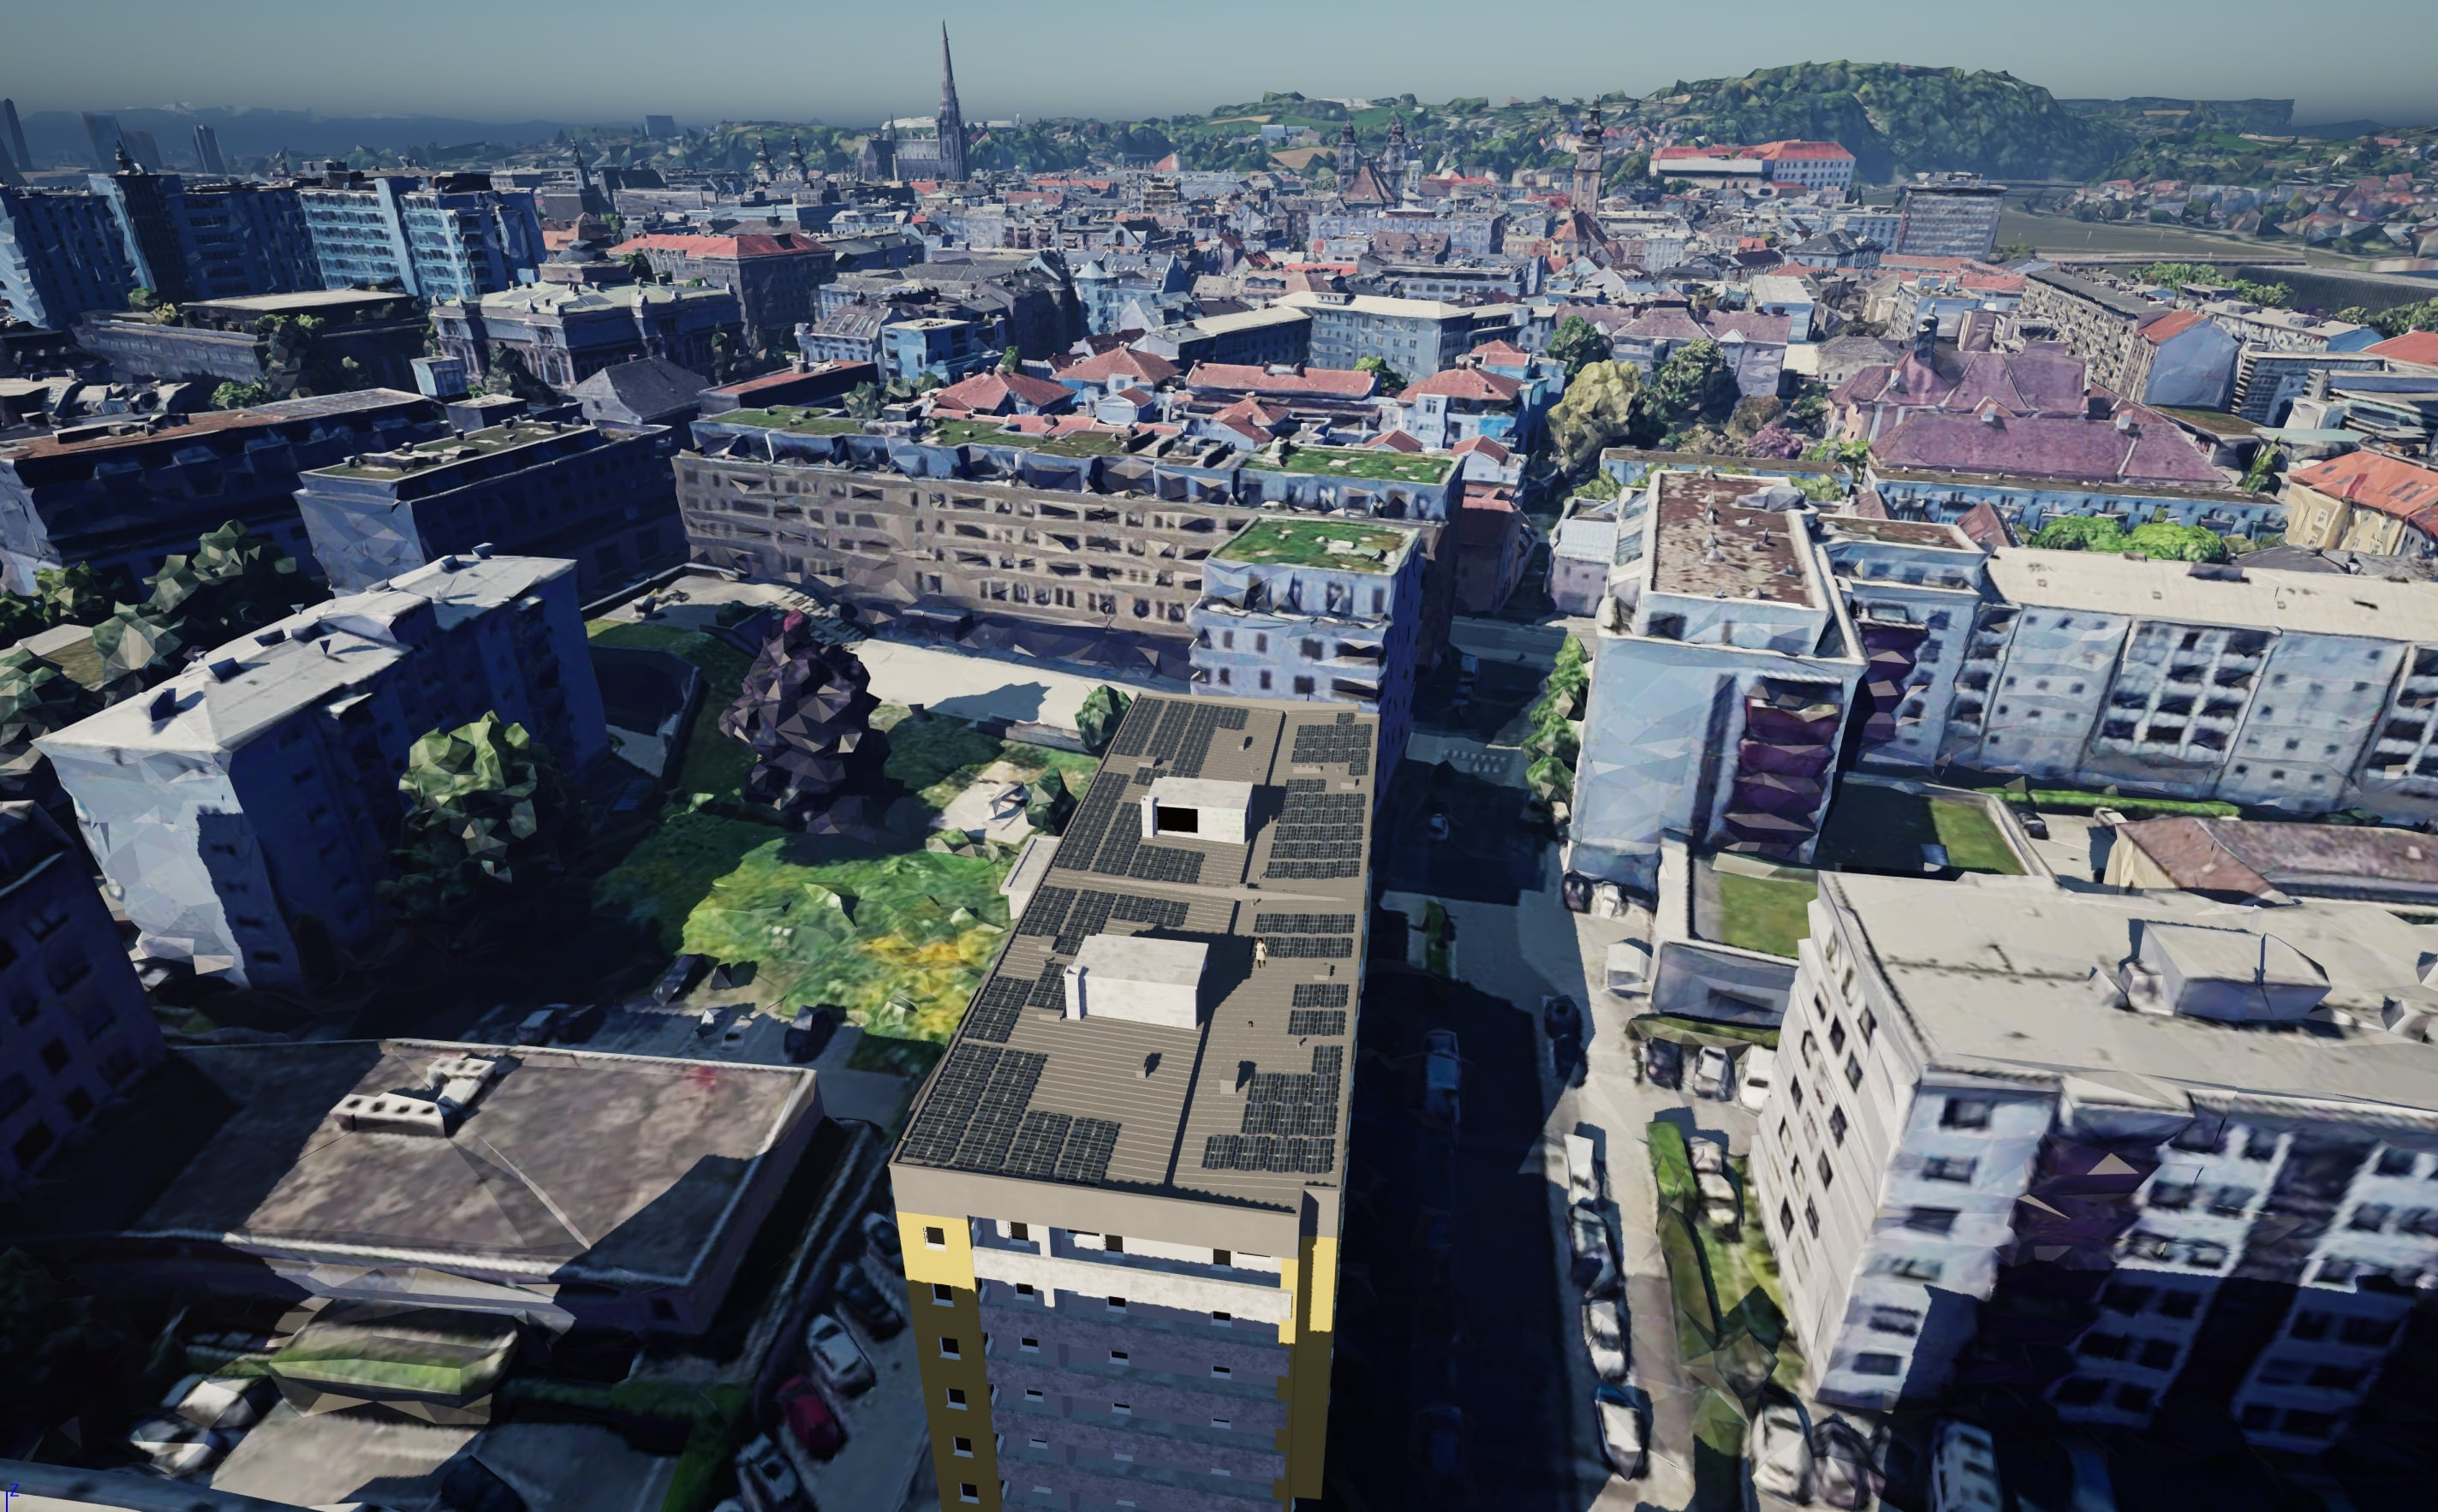
\includegraphics[width=\textwidth]{graphics/vista.jpg}
    \caption{Panoramic view of the virtual environment in \textit{SolarPowerVR}, showcasing the rooftop, the city of Linz, the Danube River, and the Alps in the distance.}
    \label{fig:environment-vista}
\end{figure}

\textbf{Navigation and Controls:} Users can navigate the rooftop environment using a teleportation mechanic, visualized by an aiming arc (Figure \ref{fig:teleport-visualization}). This minimizes motion sickness and provides a comfortable navigation experience, addressing a key challenge in VR design \cite{Winn2002Immersion}. An in-game button mapping overlay is available to remind users of the available controls (Figure \ref{fig:button-mapping}).

\begin{figure}
    \centering
    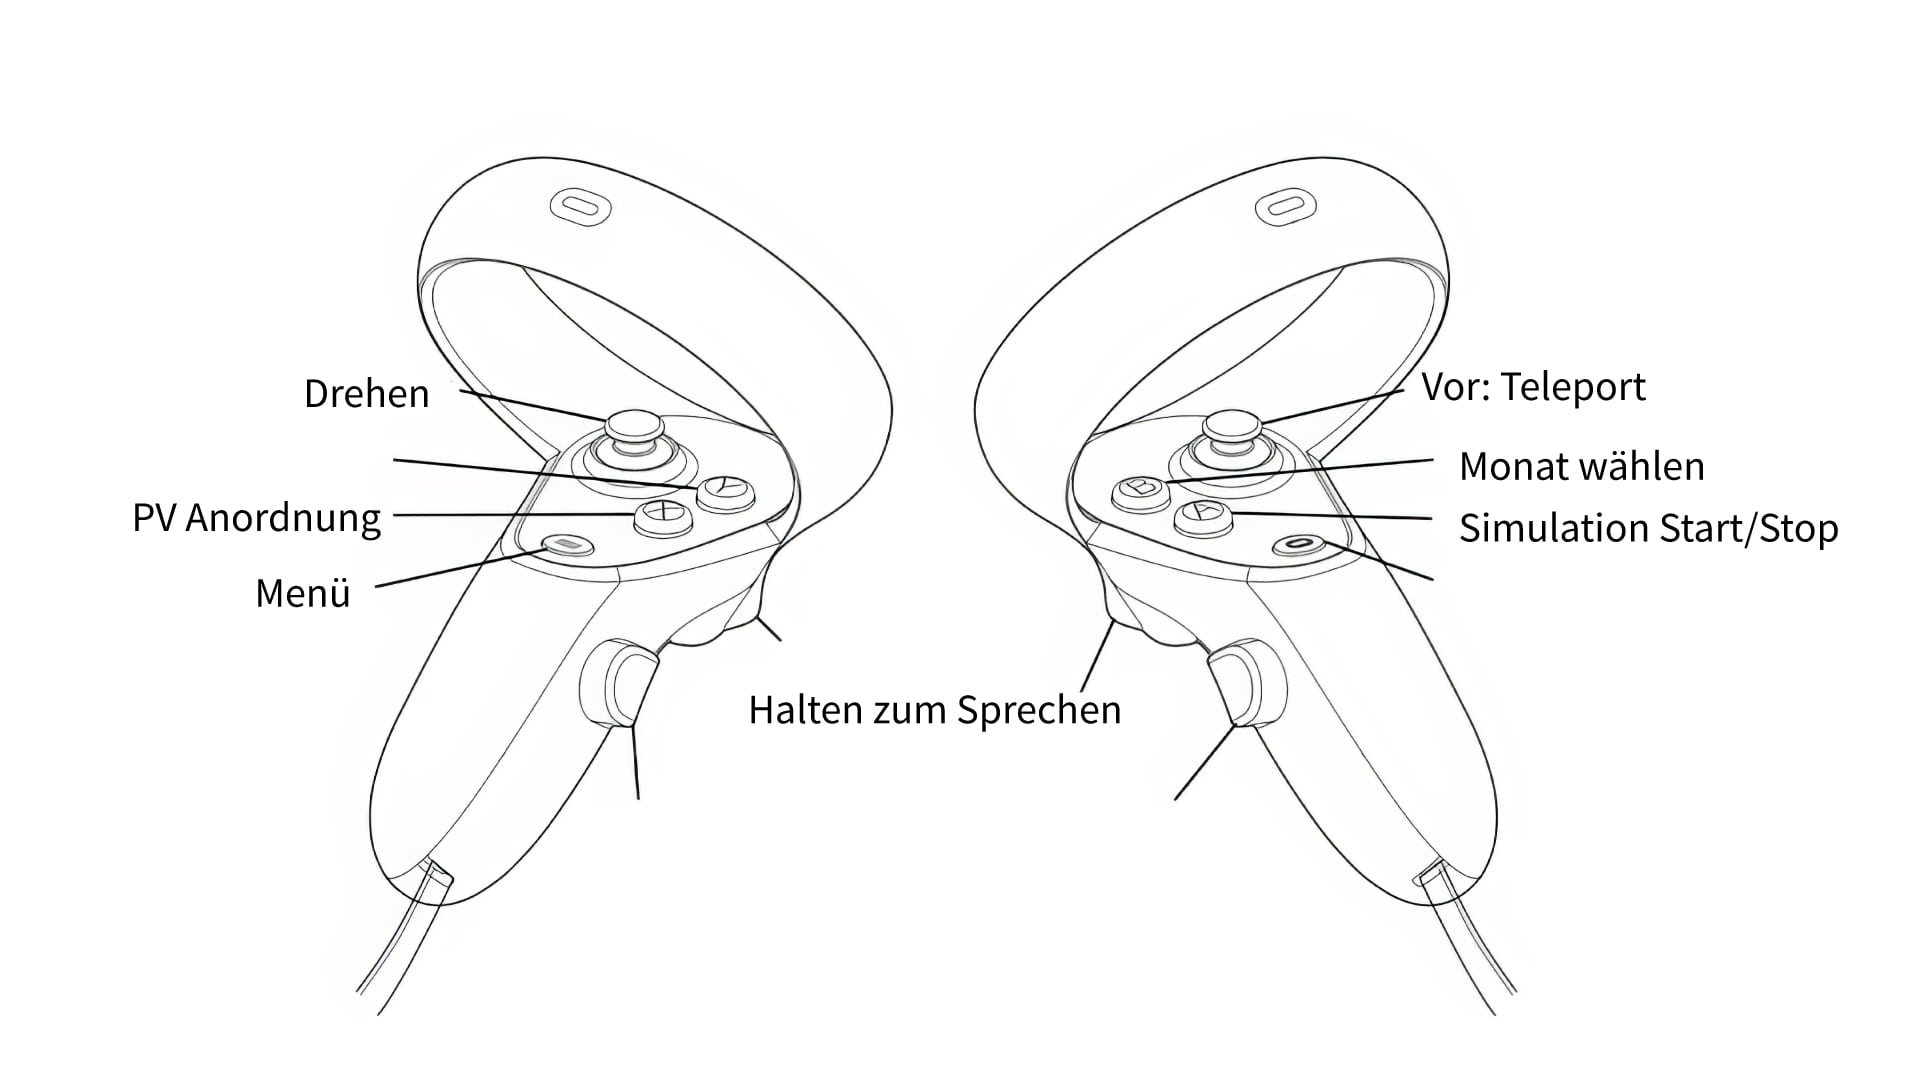
\includegraphics[width=\textwidth]{graphics/button-map.jpg}
    \caption{The in-game button mapping overlay, providing users with a visual reminder of the available controls.}
    \label{fig:button-mapping}
\end{figure}

\begin{figure}
    \centering
    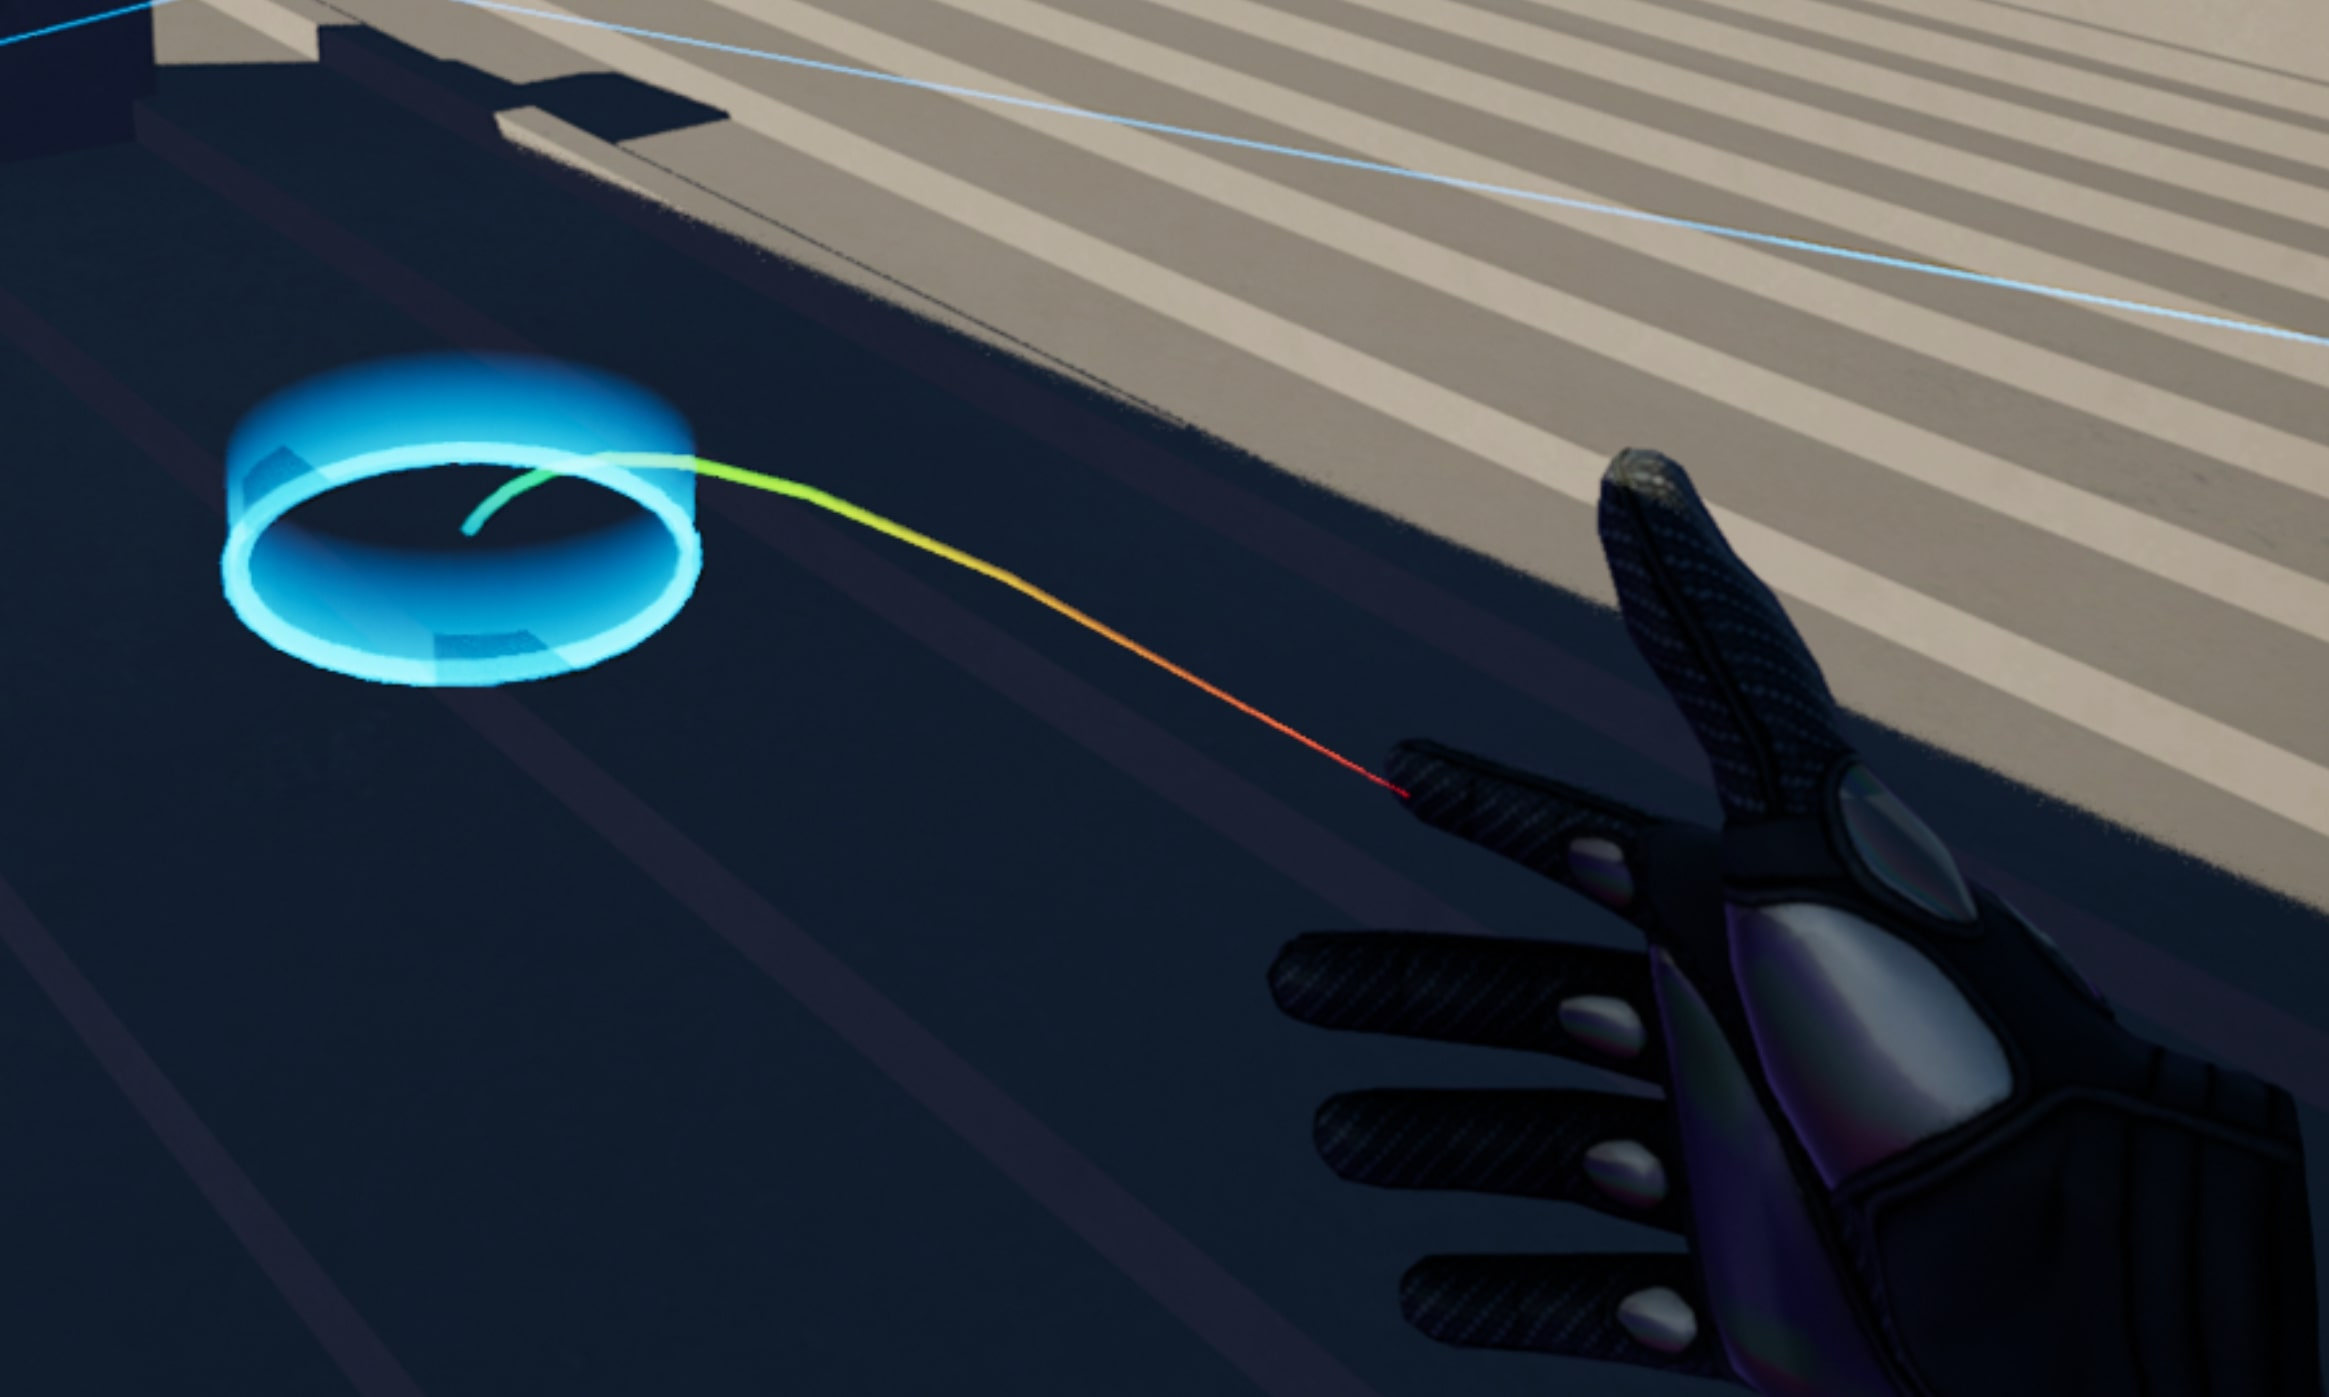
\includegraphics[width=\textwidth]{graphics/teleport.jpg}
    \caption{Visualization of the teleport aim, indicating the user's intended destination on the rooftop.}
    \label{fig:teleport-visualization}
\end{figure}

\textbf{AI Assistant:} an AI-powered assistant character accompanies the user on the rooftop. This assistant was intended to enhance the learning experience by providing guidance and information, aligning with the pedagogical benefits of incorporating avatars within EVEs to support and guide learners \cite{Mikropoulos2011VrEducational}. The design envisioned a fully functional and context-aware assistant capable of providing personalized guidance and feedback based on user actions and progress. However, limitations with the underlying Unreal Engine plugin used for AI integration (\textit{Convai}) prevented the full realization of this vision. Consequently, the AI assistant feature was removed from later versions of the application.

\begin{figure}
    \centering
    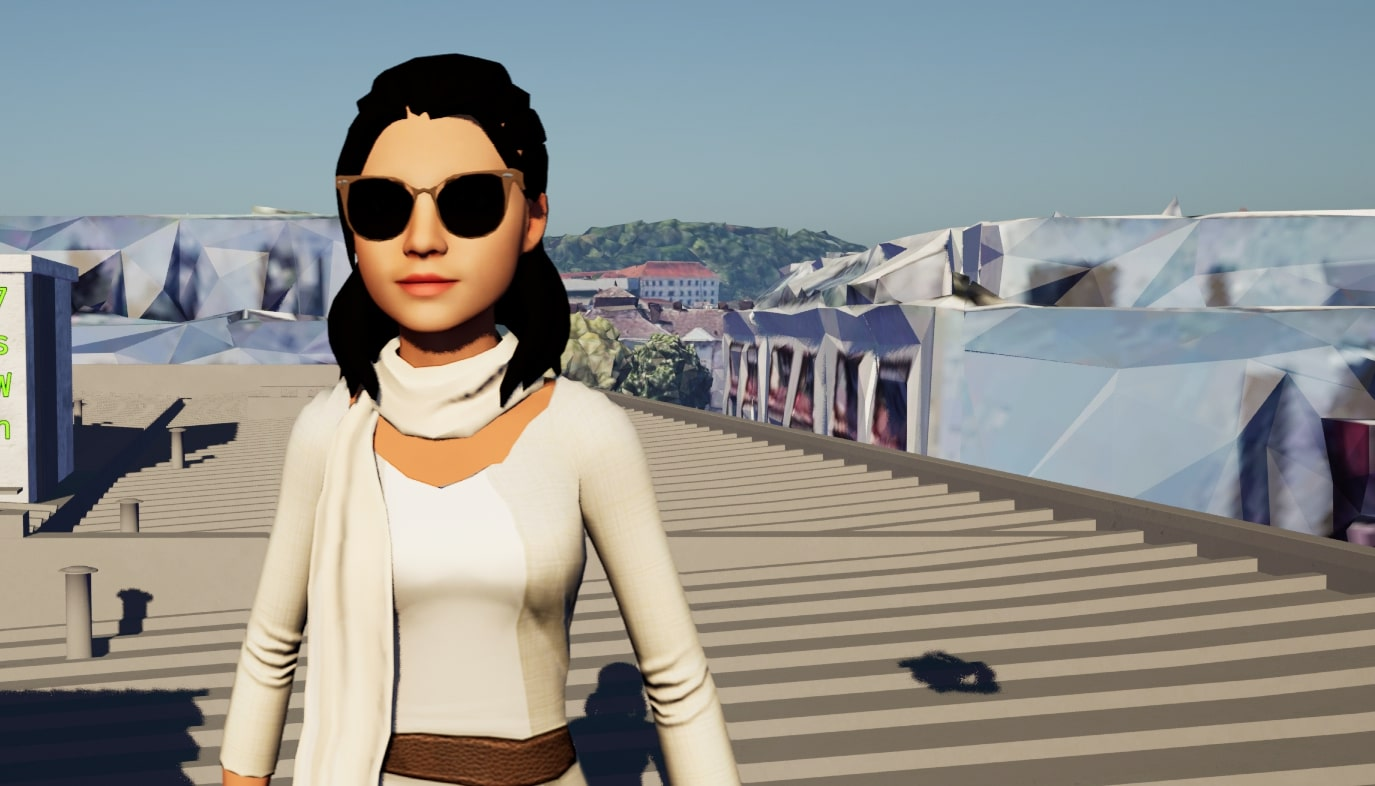
\includegraphics[width=\textwidth]{graphics/ai.jpg}
    \caption{Avatar of the AI assistant}
    \label{fig:ai-avatar}
\end{figure}

\textbf{PV Panel Configurations:} Initially, there are no PV panels installed on the roof. The user can cycle through three pre-designed PV setups by pressing a button (Figure \ref{fig:pv-configurations}):

\begin{itemize}
    \item \textbf{Flat Layout:} This configuration features the highest number of panels (150) due to their tight, shadow-minimizing arrangement. It also offers minimal wind resistance, a factor considered by the SolarProTool used in designing these layouts.
    \item \textbf{30-Degree South Inclined Layout:} This setup, with 100 panels, captures more sunlight during the winter months when the sun's trajectory is lower.
    \item \textbf{East-West Inclined Split Layout:} This configuration utilizes 90 panels inclined at 15 degrees, maximizing sun capture during morning and evening hours when energy consumption typically peaks. However, it demonstrates that this setup still cannot compete with the flat layout's higher panel count and overall energy generation.
\end{itemize}

\begin{figure}
    \centering
    \begin{subfigure}[b]{0.32\textwidth}
        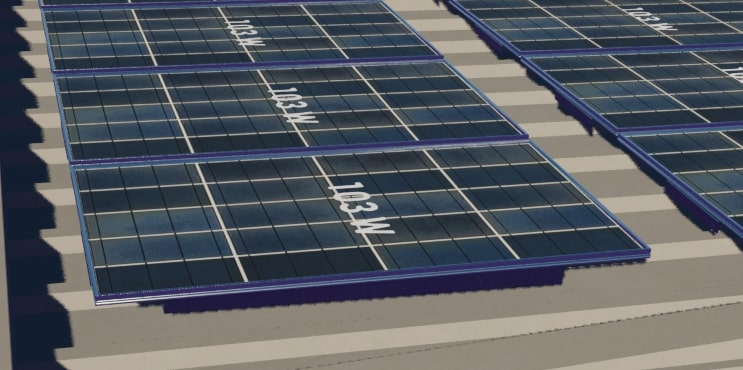
\includegraphics[width=\textwidth]{graphics/layout-flat.jpg}
        \caption{Flat Layout}
        \label{fig:flat-layout}
    \end{subfigure}
    \hfill
    \begin{subfigure}[b]{0.32\textwidth}
        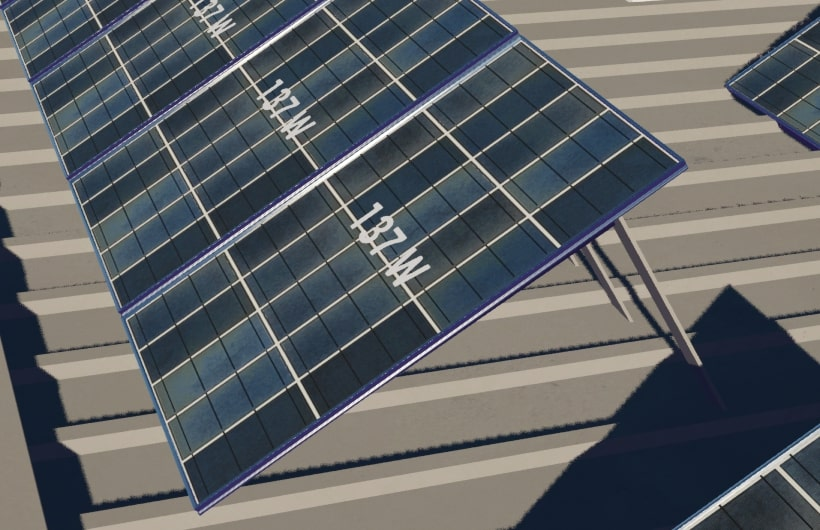
\includegraphics[width=\textwidth]{graphics/layout-south.jpg}
        \caption{South Inclined Layout}
        \label{fig:south-layout}
    \end{subfigure}
    \hfill
    \begin{subfigure}[b]{0.32\textwidth}
        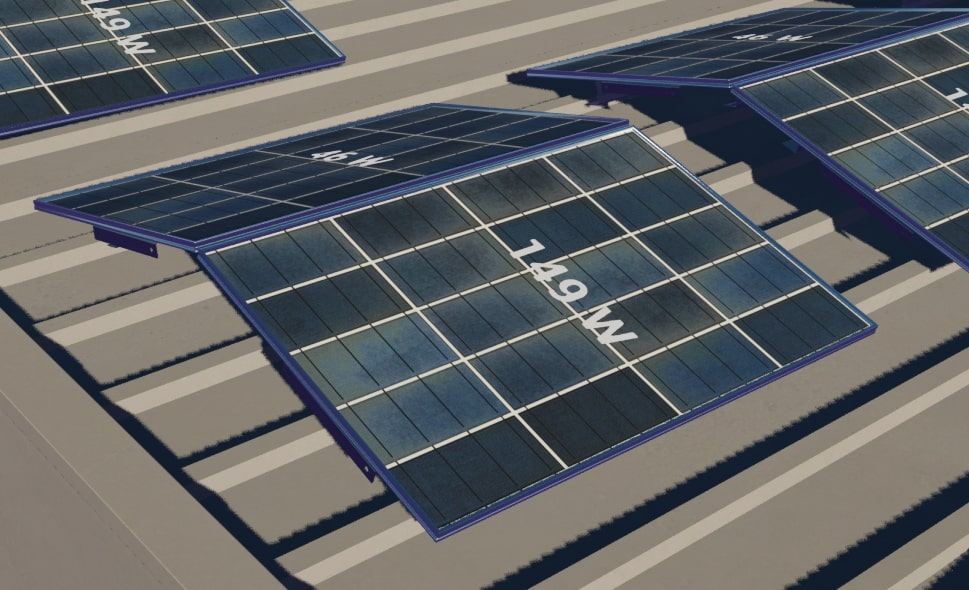
\includegraphics[width=\textwidth]{graphics/layout-eastwest.jpg}
        \caption{East-West Split Layout}
        \label{fig:east-west-layout}
    \end{subfigure}
    \caption{The three available pre-designed PV panel configurations.}
    \label{fig:pv-configurations}
\end{figure}

These configurations allow users to explore different design considerations and their impact on energy production, fostering constructivist learning through experimentation \cite{Mikropoulos2011VrEducational}.

\textbf{Simulation Controls:}

\begin{itemize}
    \item \textbf{Month Advancement:} A button allows the user to increment the month of the simulation, starting from the summer solstice.
    \item \textbf{Simulation Start/Stop:} Another button starts and stops the simulation. Upon starting, the time is automatically set to sunrise, allowing the user to witness the entire day's energy production cycle.
\end{itemize}

These controls provide users with agency and control over the simulation, allowing them to manipulate variables and observe the outcomes, further supporting active learning \cite{Dalgarno2010Learning}.

\textbf{Simulation Feedback:} Three widgets are strategically placed on the lift housing walls, ensuring visibility from various points on the rooftop  (Figure \ref{fig:simulation-feedback}):

\begin{itemize}
    \item \textbf{The Clock:} Displays simulation input parameters such as date, time, number of panels deployed, current kilowatt (kW) output, and accumulated kilowatt-hours (kWh) for the day.
    \item \textbf{Panel Power Output:} Each panel displays its current power output in Watts.
    \item \textbf{Line Graph:} Shows curves representing the kW output for each simulated day, with time on the x-axis and kW on the y-axis. Each curve is color-coded for easy differentiation.
    \item \textbf{Bar Graph:} Presents a bar for each simulated day, with the bar's height reflecting the accumulated kWh for that day.
\end{itemize}

\begin{figure}
    \centering
    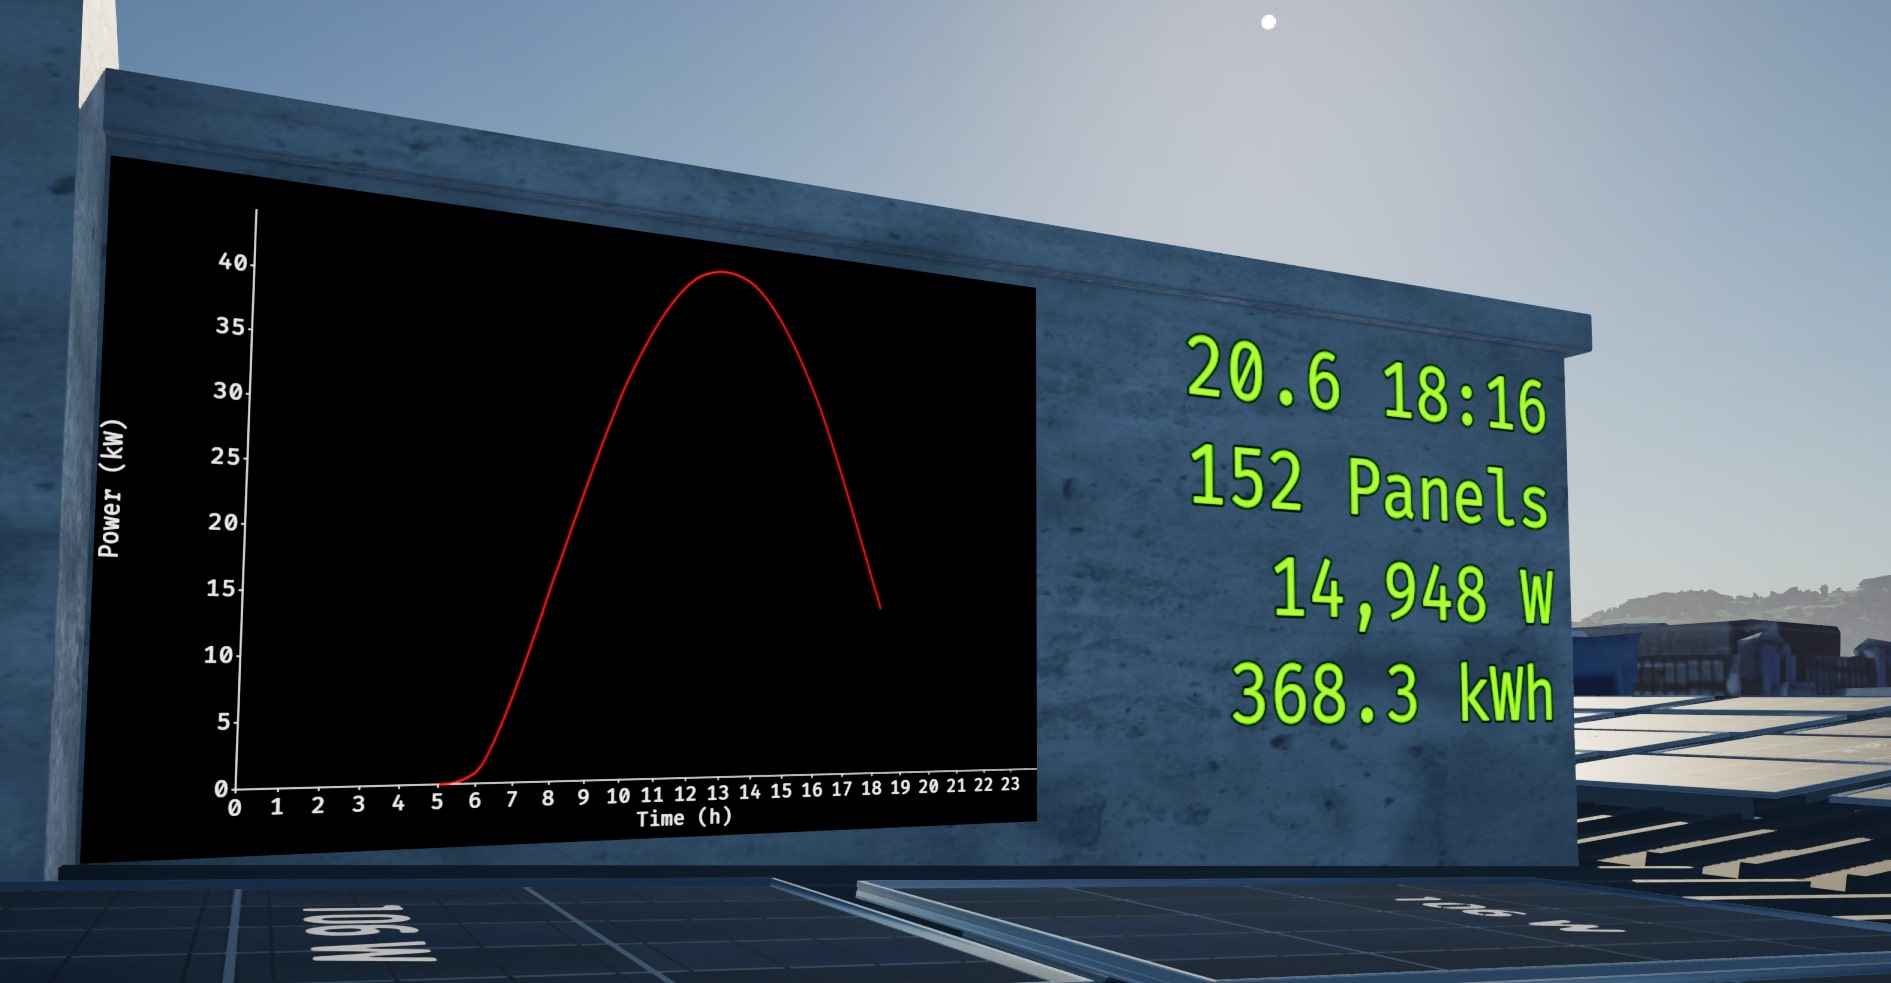
\includegraphics[width=\textwidth]{graphics/clock-power.jpg}
    \caption{The clock widget and line graph in \textit{SolarPowerVR}, providing real-time feedback on the PV system's performance.}
    \label{fig:simulation-feedback}
\end{figure}

These widgets provide clear and concise feedback on the performance of the PV system, enhancing understanding and supporting knowledge construction \cite{Merchant2014VrEffectiveness, Mikropoulos2011VrEducational, Sung2015Effects}.

By incorporating research-backed design principles and leveraging the immersive capabilities of virtual reality, \textit{SolarPowerVR} offers a focused and accessible platform for learning about PV systems, contributing to a greater understanding and acceptance of renewable energy technologies.

\chapter{Implementation}

This chapter details the implementation of \textit{SolarPowerVR}, a virtual reality application designed to enhance public understanding of PV systems and promote their adoption in Austria. The chapter outlines the development environment, software architecture, simulation implementation, user interface and interaction design, testing and validation procedures, performance optimization strategies, and deployment process.

\section{Development Environment}


\textit{SolarPowerVR} was developed using \href{https://www.unrealengine.com/de}{Unreal Engine} (UE) 5.2 to 5.4, chosen for its robust rendering capabilities, extensive plugin ecosystem, and support for virtual reality platforms. The application was programmed using a combination of UE Blueprints for visual scripting and C++ for performance-critical components. This mixed approach allows for optimized performance and design flexibility. C++ development and compilation were performed using \href{https://visualstudio.microsoft.com/de/vs/community/}{Visual Studio 2022 Community Edition}. The following tools were utilized to enhance the development environment:

\begin{itemize}
    \item \href{https://dev.epicgames.com/documentation/en-us/unreal-engine/geographically-accurate-sun-positioning-tool-in-unreal-engine?application_version=5.4}{SunPosition} plugin: provides accurate simulation of the sun's position based on date, time, and geographic location, and was extended for our use case to calculate solar irradiance.
    \item \href{https://github.com/kamrann/KantanCharts}{KantanCharts} plugin: facilitated the creation of charts for visualizing simulation data, enabling users to analyze and compare the performance of different PV system configurations.
    \item \href{https://developers.google.com/maps/documentation/tile/3d-tiles-overview}{Google 3D Tiles}: provides realistic static meshes of the environment, allowing for stunning perspective views and immersive storytelling.
    \item \href{https://cesium.com/platform/cesium-for-unreal/}{Cesium} plugin: was used to stream realistic environments from Google 3D Tiles. However, it had performance issues that led to its eventual replacement.
    \item \href{https://www.unrealengine.com/marketplace/en-US/product/convai}{Convai} plugin: enabled the integration of an AI character that could interact with users, provide voice responses, and animate accordingly, but ultimately required tighter coupling with the game state to be effective.
    \item \href{https://www.blender.org/}{Blender} 4.1 with \href{https://prochitecture.gumroad.com/l/blender-osm}{Blosm} plugin: allowed for the import of Google 3D Tiles into Blender, enabling the creation of optimized static meshes for the game environment, with six levels of quality.
\end{itemize}

\section{Software Architecture}

\textit{SolarPowerVR} is built using a modular architecture, with each class responsible for a specific set of functionalities. This design approach enables easy maintenance, modification, and extension of the simulation. Blueprints inherit from C++ classes, allowing for a mixed approach within the Unreal Engine architecture. This provides both optimized performance and design flexibility. The core classes are:

\begin{itemize}
    \item \lstinline|ASimulationGameMode|: This class serves as the central manager of the simulation, responsible for updating the sun's position, irradiance, and solar panel wattage each frame. It provides an interface for the users pawn to interact with the simulation, allowing for changes to the simulation's time and date and pv layout selection.
    \item \lstinline|ASolarPanel|: Implemented in C++, this class represents a single solar panel, with properties such as nominal wattage (default 400W) and current power output. The class calculates its power output based on the irradiance received and its orientation relative to the sun. The class is extended in \lstinline|BPSolarPanel| to provide additional level design capabilities: the tilt of the panel and the visibility of the stands can be adjusted through actor settings in the level design, allowing for flexibility in the simulation.
    \item \lstinline|BPSunSky|: Implemented in Blueprints and extending the SunPosition plugin, this class simulates the sun's position based on the current time, date, and the latitude and longitude of Linz. It then calculates the Airmass and irradiance, providing a realistic and accurate representation of the sun's behavior. The correction curves were implemented in Blueprints to allow for easier experimentation when aligning the theoretical output with the more realistic SolarProTool simulation results.
    \item \lstinline|BPVrPawn|: Implemented in Blueprints and building upon the UE VR template pawn, this class represents the player character and handles all interactivity within the simulation. It uses the interface provided by the \lstinline|ASimulationGameMode| class to interact with the simulation, and also handles movement, displays the button mapping, and facilitates voice interactions with the AI.
\end{itemize}

A key aspect of the architecture is the decoupling of the classes, which allows for easier modification, iteration, and testing. By avoiding tight coupling, changes to one class do not have a ripple effect on the others, making it easier to refine and extend the simulation.

\section{Simulation Interface and User Interaction Mechanisms}

The simulation interface is designed to provide an intuitive and user-friendly experience for exploring photovoltaic systems. The interface consists of several key elements:

\begin{itemize}
    \item \textbf{Clock Widget:} The clock widget displays the current date, time, number of active solar panels, total power output (Watts), and total energy generated (Watt-hours). This information is updated every frame to reflect the current simulation state. The clock widget provides a quick and easy way for users to monitor the performance of the photovoltaic system.
    \item \textbf{Line Graph:} The line graph displays the power output (Watts) of each photovoltaic system layout over time. This allows users to compare the performance of different configurations and identify trends in energy production. The line graph is updated every frame to reflect the current simulation state.
    \item \textbf{Bar Chart:} The bar chart displays the total energy generated (Watt-hours) for each layout and month. This provides a visual representation of the long-term performance of different configurations and allows users to identify areas for improvement. The bar chart is updated at the end of each simulated day.
\end{itemize}

Users interact with the simulation through a VR headset and controllers. The primary interaction mechanisms include:

\begin{itemize}
    \item \textbf{Teleportation:} Users can teleport to different locations within the virtual environment to explore the photovoltaic system from various perspectives. This is implemented using UE's built-in VR teleportation functionality and provides a convenient way for users to navigate the simulation environment.
    \item \textbf{Layout Selection:} Users can switch between different photovoltaic system layouts (flat, south-facing, east/west split) to observe the impact of panel orientation on power output. This is triggered by a button press on the VR controller and handled by the `NextLayout` function in the `SimulationGameMode` class.
    \item \textbf{Month Selection:} Users can increment the month to observe the effects of seasonal variations on photovoltaic system performance. This is triggered by pressing a button on the controller and handled by the VRPawn, which calls the GameMode.
    \item \textbf{Simulation Control:} Users can start, stop, and reset the simulation using dedicated buttons on the VR controller. These actions are handled by the `StartSimulation`, `StopSimulation`, and `ResetSimulation` functions in the `SimulationGameMode` class.
    \item \textbf{Button Map Visibility:} Users can toggle the visibility of a button map overlay, providing a reminder of the available controls. This is triggered by a button press on the VR controller.
\end{itemize}

\section{Simulation}

The simulation uses a tick-based system, updating the simulation state each frame. \lstinline|SimulationGameMode| orchestrates the simulation loop, updating the sun's position and irradiance based on the current time and date. It allows users to run the simulation in time-lapse to observe the effects of different PV panel configurations over the day. This is achieved by multiplying the time elapsed between frames (deltaTime) with a fixed speed factor.

The core of the simulation lies in the calculation of solar irradiance, which is influenced by the sun's position on the sky, atmospheric conditions, and seasonal variations. \lstinline|BPSunSky| uses the SunPosition plugin to accurately simulate the sun's position based on the current time and date. This is then used to calculate the airmass and then to calculate the theoretical irradiance, which is further corrected for seasonal variations using 3 empirical correction curves. While this empirical approach is effective, there is potential for future optimization by developing an algorithmic approach to align simulation output with SolarProTool data.

\paragraph{\lstinline|updateAirmass()|} calculates the air mass ($AM$) based on the solar zenith angle ($\theta_z$) using the Kasten and Young model \cite{Kasten1989airmass}. This model provides a reliable approximation of $AM$ by accounting for atmospheric conditions and the path length of sunlight through the atmosphere.

First, the solar zenith angle is derived from the inversed elevation angle provided by the SunPosition plugin using an inversion transformation:

\begin{equation} \label{eq:theta_z}
\theta_z = 180^\circ + 90^\circ - \text{elevation\_inv}
\end{equation}

This transformation aligns the plugin's output with the standard definition of the solar zenith angle. Subsequently, the air mass is calculated as follows:

\begin{equation} \label{eq:airmass}
AM = \frac{1}{\cos(\theta_z) + 0.50572 \cdot (96.07995 - \theta_z)^{-1.6364}}
\end{equation}

Figure \ref{fig:corrected-airmass} illustrates the non-linear relationship between the corrected air mass and the zenith angle. This accurate AM value is crucial for simulating the attenuation of solar radiation through the atmosphere. Figure \ref{fig:airmass-bp} shows the blueprint implementation of equation \ref{eq:airmass}.

\begin{figure}[h]
    \centering
    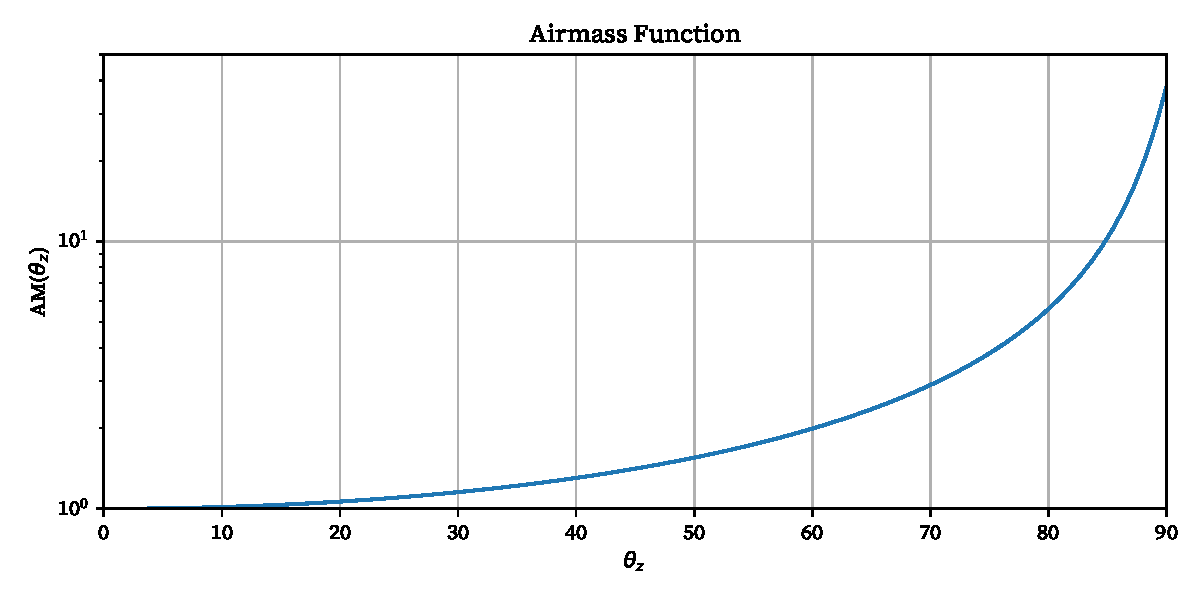
\includegraphics[width=\textwidth]{graphics/airmass.pdf}
    \caption{Corrected air mass as a function of the zenith angle ($\theta_z$), plotted over a range from 0 to 90 degrees.}
    \label{fig:corrected-airmass}
\end{figure}

\begin{figure}
    \centering
    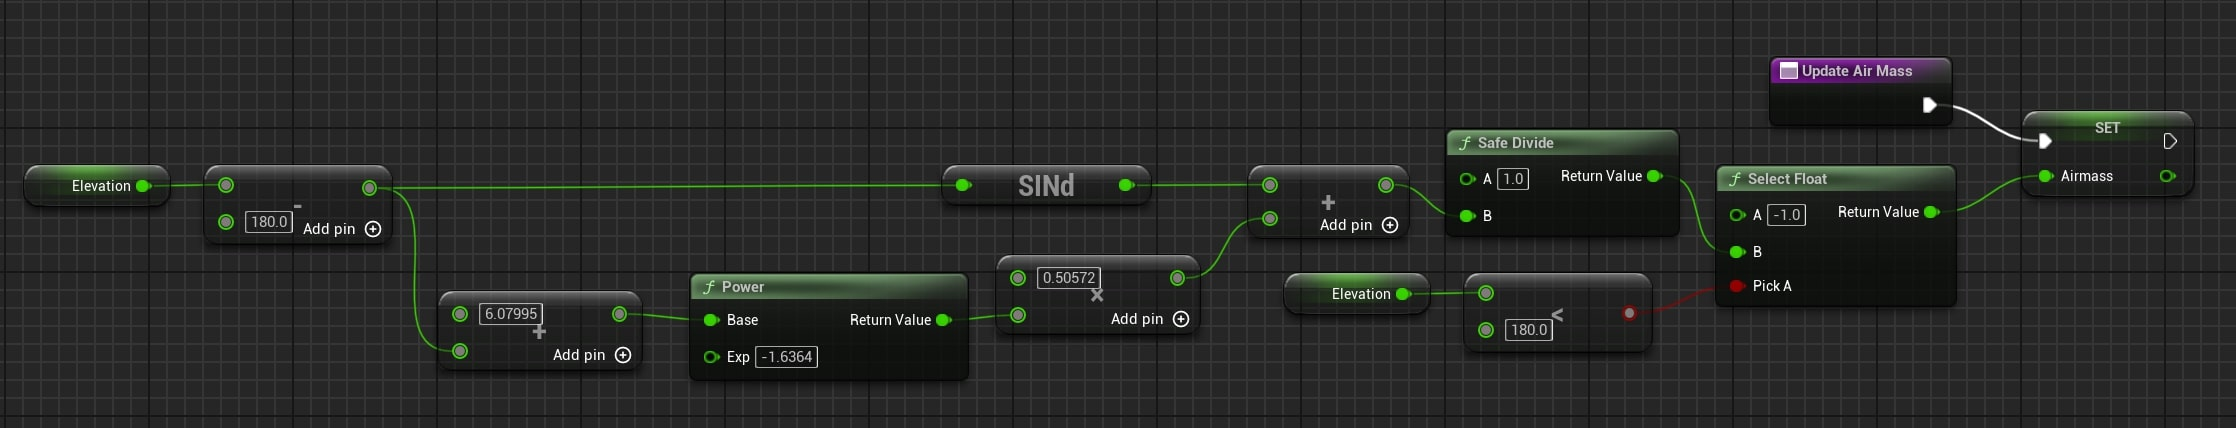
\includegraphics[width=\textwidth]{graphics/airmass-bp.jpg}
    \caption{Blueprint implementation for calculating the airmass}
    \label{fig:airmass-bp}
\end{figure}


\paragraph{\lstinline|updateIrradiance()|} calculates the solar irradiance based on the calculated air mass, utilizing the experimentally determined equation \ref{eq:irradiance} from Meinel and Meinel \cite{Meinel1976irradiance}. $I_D$ represents the direct component of sunlight intensity on a plane perpendicular to the sun's rays (kW/m$^2$). $AM$ is the calculated air mass. The solar constant is represented by 1.353 kW/m$^2$, while the factor 0.7 approximates the transmission of solar radiation through the atmosphere. The exponent 0.678 is a correction factor accounting for atmospheric layer non-uniformities.

\begin{equation} \label{eq:irradiance}
I_D = 1.353 \cdot 0.7^{AM^{0.678}}
\end{equation}

Figure \ref{fig:irradiance} depicts the relationship between irradiance, air mass, and zenith angle, highlighting the decrease in irradiance with increasing air mass and zenith angle due to scattering and absorption of sunlight.

\begin{figure}[h]
    \centering
    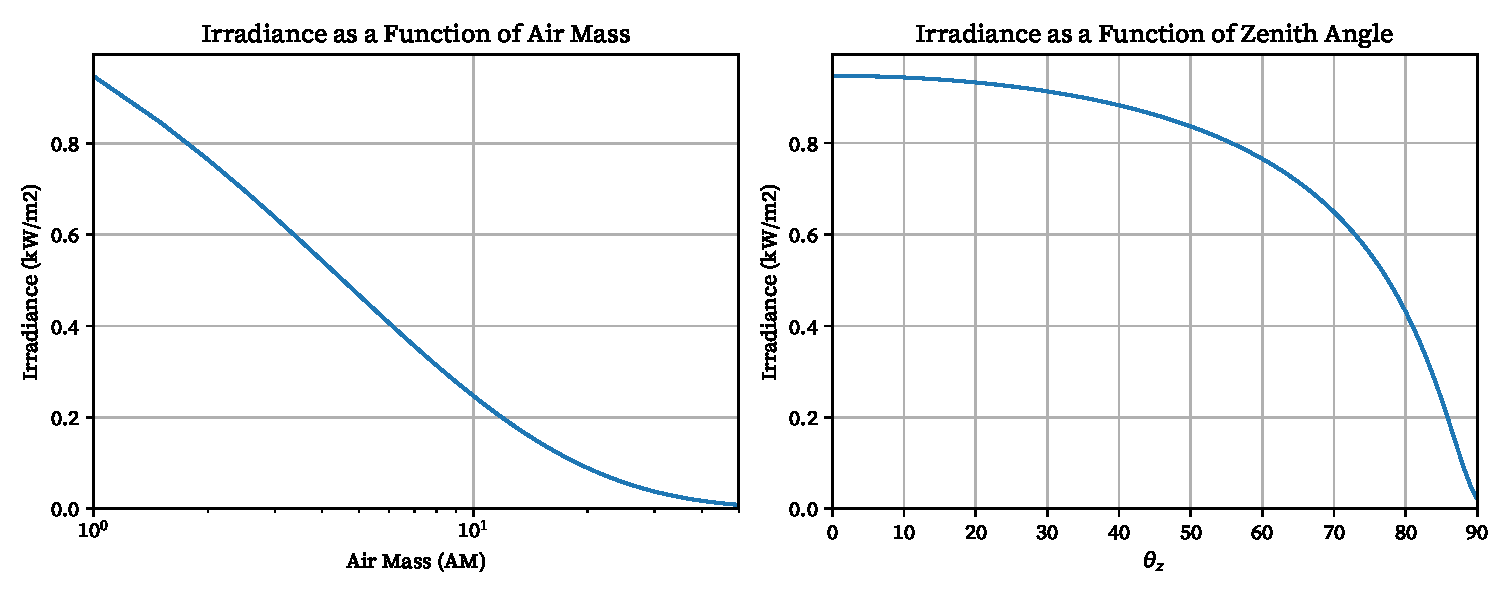
\includegraphics[width=\textwidth]{graphics/irradiance.pdf}
    \caption{Irradiance as a function of air mass (left) and zenith angle (right), demonstrating the decrease in irradiance with increasing values.}
    \label{fig:irradiance}
\end{figure}

\begin{figure}
    \centering
    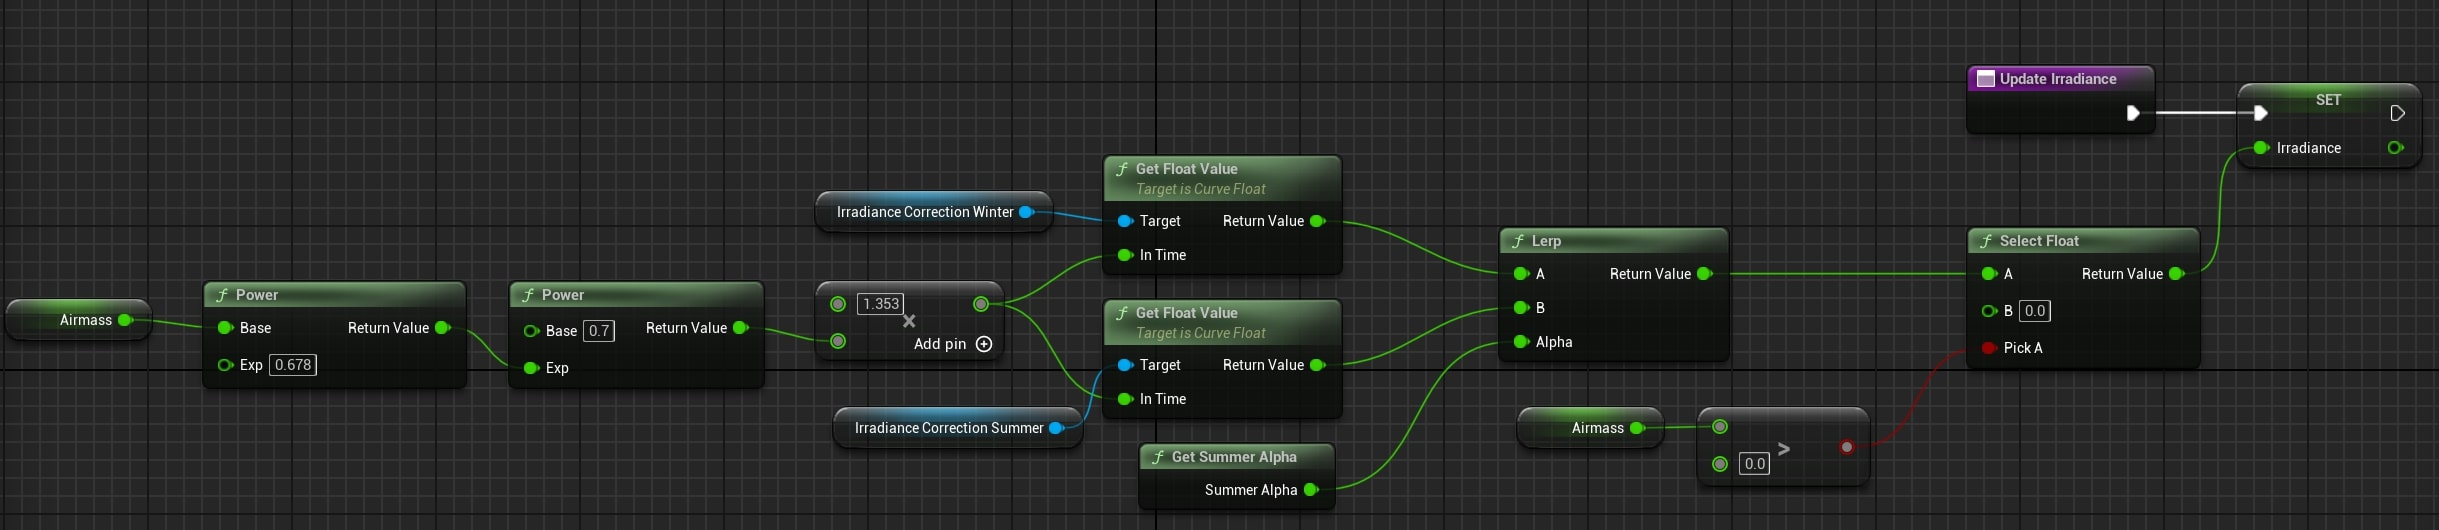
\includegraphics[width=\textwidth]{graphics/irradiance-bp.jpg}
    \caption{Blueprint implementation for calculating the irradiance}
    \label{fig:airmass-bp}
\end{figure}

\paragraph{Seasonal Correction}

Calculating solar irradiance ($I_D$) under optimal conditions can lead to inaccuracies in power output predictions. To address this, we designed a seasonal correction factor ($I_C$), modulated by the day of the year, based on empirical testing. This correction ensures that the simulation results closely align with those generated by SolarProTool, reflecting realistic variations in solar irradiance throughout the year and leading to more accurate power output estimations.

This seasonal correction is based on two empirically determined curves: a winter correction curve ($WinterCurve(I_D)$) and a summer correction curve ($SummerCurve(I_D)$). These curves were derived by comparing simulation output with Levasoft Solar Pro data, focusing on the winter and summer solstices, respectively. The winter correction curve utilizes a linear interpolation function defined by the points: (0,0), (0.1, 0), (0.4, 0.36), (0.5, 0.5), (0.6, 0.63). The summer correction curve is defined by another linear interpolation function with the points: (0,0), (0.3, 0.097), (0.4, 0.167), (0.7, 0.568), (0.9, 0.788), (0.92, 0.8038).

To ensure a smooth transition between these two correction curves throughout the year, an interpolation factor ($t$) is calculated using a cubic interpolation curve based on the day of the year. This factor determines the blend between the winter and summer corrections, dynamically adjusting the seasonal correction factor ($I_C$) as the year progresses.

\begin{equation} \label{eq:interpolation_factor}
t = \text{InterpolationCurve}\left(\left(\text{day}_{\text{(of the year)}} - 12\right) \mod 365\right)
\end{equation}

The cubic interpolation curve uses the points (0,0), (80, 0.853), (180, 1), (285, 0.853), and (365,0). The corrected irradiance ($I_C$) is then determined by blending the winter and summer irradiance curves based on the interpolation factor ($t$):

\begin{equation} \label{eq:seasonal_irradiance}
I_C = \text{WinterCurve}(I_D) \cdot (1 - t) + \text{SummerCurve}(I_D) \cdot t
\end{equation}

Figure \ref{fig:seasonal_correction_curves} illustrates the seasonal correction curves and their interpolation.

\begin{figure}[h]
    \centering
    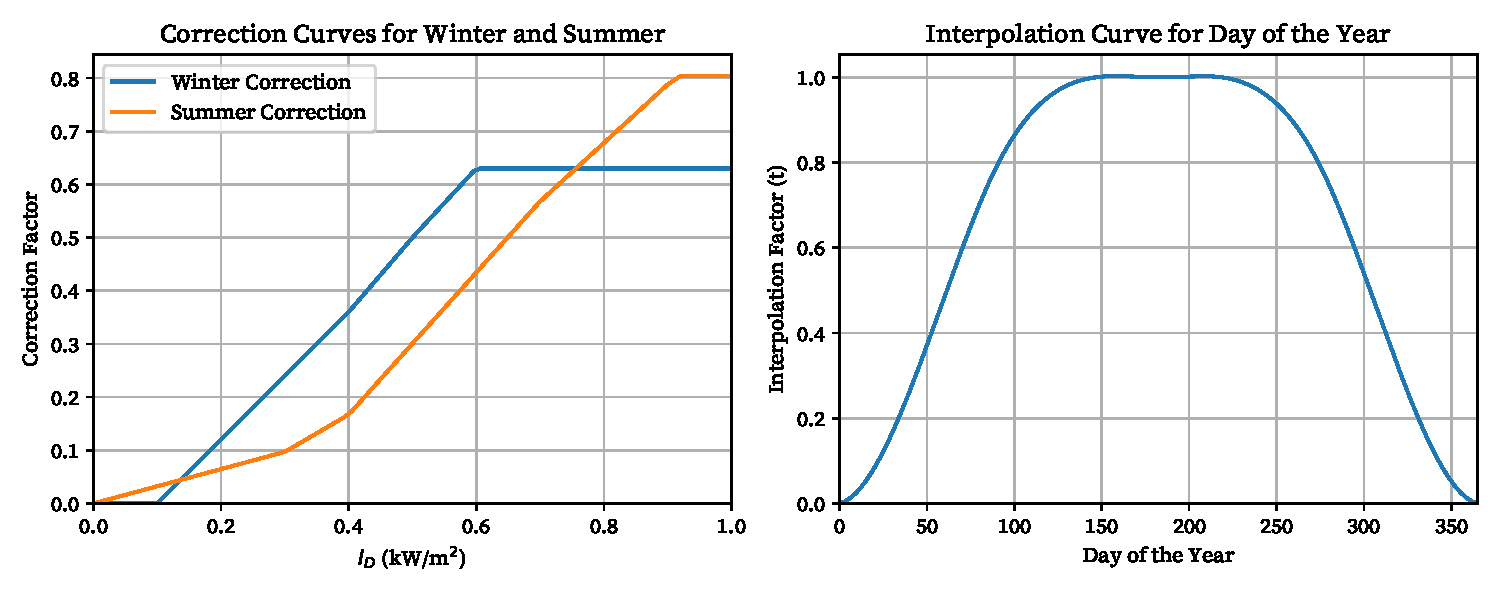
\includegraphics[width=\textwidth]{graphics/correction.pdf}
    \caption{Seasonal correction curves, showing the interpolation between the winter and summer correction curves. Left: The winter and summer correction curves as functions of the irradiance. Right: The interpolation factor as a function of the day of the year.}
    \label{fig:seasonal_correction_curves}
\end{figure}

This approach ensures that the simulated irradiance values closely match the expected values for Linz, Austria, throughout the year, enhancing the realism and accuracy of the \textit{SolarPowerVR} simulation.

\lstinline|SolarPanel| then calculates its power output based on the received irradiance and its orientation relative to the sun using the following formula:

\begin{equation}
    \text{Watt} = \cos(\theta) \cdot \text{NominalWatt} \cdot \text{Irradiance}
\end{equation}

where $\theta$ is the angle between the panel's normal vector and the sun direction vector.

This data is then visualized as a label on the PV panel and aggregated using KantanCharts UI components, providing users with real-time feedback on the performance of the PV system.

\section{Performance Optimization}

To achieve a stable 90 frames per second (fps) on the target hardware (mobile RTX 4090), we conducted a thorough performance optimization process. Our goal was to minimize computational overhead while maintaining visual fidelity. Through these optimizations, we significantly improved frame times and enhanced the stability of the application, ensuring a smooth and responsive user experience.

One of the major performance bottlenecks was the Cesium plugin, which required 5ms alone to evaluate which tiles to show and did so on the game thread. This was not only too expensive, but also unnecessary. By replacing the Cesium plugin with static mesh assets, we zeroed the computational load associated with dynamic tile loading. Additionally, this allowed us to take advantage of Nanite optimization, which helped reduce overdraw.

We also optimized the simulation loop by migrating it from Blueprints to C++. This provided a substantial performance boost, as the iteration over 350 panels per frame was no longer a bottleneck.

To further optimize rendering performance, we merged tiles to reduce the number of draw calls and actors in the scene. Although this made frustrum culling less effective, it was a trade-off to achieve the desired performance.

Another key optimization was tweaking the Virtual Shadow Maps (VSM) settings. As the highest fidelity shadows available in UE with software raytracing, VSMs are extremely expensive with a moving light source. However, by adjusting the max shadow distance and resolution, we found a compromise that balanced visual quality and performance.

Finally, we disabled tick on environment assets, as they do not require per-frame updates, which saved cpu time.

\section{Testing and Validation}

The application was continuously tested to ensure functionality and accuracy. This included logging and analyzing simulation data to identify and resolve any discrepancies. Manual tests were conducted regularly to verify navigation, layout selection, simulation controls, and data visualization. A test session with one participant provided valuable feedback on the usability and effectiveness of the application. This feedback led to the implementation of the button map overlay \ref{fig:button-mapping} to improve the user's understanding of the available controls.

\section{Accessibility}

Accessibility features for users with visual or other disabilities were not explored in this study. However, optimization for colorblindness seems reasonable.

\section{Deployment}

To ensure a great experience for the workshop attendees, we carefully planned and executed the deployment of the application to the target hardware. Some laptops were fresh out of the box, so we started by installing the latest Windows updates to ensure a stable operating system. We then manually installed the chipset drivers to support the full USB 3.2 speeds required to achieve the desired resolution and frame rate. We also installed the latest NVIDIA drivers and Oculus software.

To optimize the Oculus experience, we used the Oculus Debug Tool to override some settings and achieve the best possible quality. Specifically, we set the screen resolution to 100\% for a clear image, disabled automatic frame generation to prevent image artifacts and receive a dynamic frame rate. We set the distortion to low and the encoding to H265, which provided better image quality without introducing any noticeable lag. Finally, we disabled the sharpening effect, which caused flickering in our tests.

To ensure that the application would work seamlessly in the event of a link failure, we enabled "Link USB Auto Connect" in the headset's developer settings. This allowed us to simply unplug and replug the headset to reconnect without requiring any user action.

After completing these steps, we tested each machine to ensure that the deployment was successful and the application was running smoothly. However, we experienced some problems with the Quest 2 devices, which would occasionally fail. Despite rebooting the PC and headsets, we were unable to determine the root cause of the problem. We did find that it was important to use a high quality cable, as some cables may have had defects that contributed to the problems. In contrast, the Quest 3 unit performed reliably, suggesting that it may be a more robust hardware platform.

\chapter{Evaluation}

This chapter outlines the evaluation process of the two virtual reality (VR) applications, \textit{KaisergasseVR} and \textit{SolarPowerVR}, to assess their effectiveness in enhancing understanding and engagement with climate-friendly technologies, particularly focusing on PV solutions. The initial evaluation focused on \textit{KaisergasseVR}, establishing a baseline understanding of user experience and learning outcomes. Building upon this baseline and user feedback, \textit{SolarPowerVR} was designed to incorporate more interactive elements and observational opportunities, aiming to further increase understanding and interest in PV solutions and impart factual knowledge through observation. The user studies were conducted after participants engaged with each VR application, with optional participation.. 

This chapter outlines the evaluation process of the two virtual reality (VR) applications \textit{KaisergasseVR} and \textit{SolarPowerVR}. The primary objective was to assess whether \textit{SolarPowerVR} could contribute more than \textit{KaisergasseVR} to participants' understanding and engagement with climate-friendly technologies, with a particular focus on photovoltaic solutions. The user studies were conducted following participants' engagement with the respective VR application. Participation in the post-experience surveys was optional.

The initial evaluation began with the \textit{KaisergasseVR} application, which served as a baseline. This user study was conducted to assess the effectiveness of a VR application in raising awareness and influencing attitudes towards climate-positive actions within an urban environment. We aimed to determine the application's effectiveness in conveying the utility of climate-friendly actions and to identify areas needing enhancement.

Building upon the established baseline and feedback, \textit{SolarPowerVR} was then designed to incorporate more interactive elements and observational opportunities to engage users. While continuing to target the primary goals of further increasing understanding and interest in PV solutions, it also aimed to additionally impart factual knowledge through observation, such as the optimal orientation of photovoltaic panels. This secondary goal explores whether deeper engagement and interactivity can contribute to more comprehensive learning outcomes.

\section{User study on \textit{KaisergasseVR}}
The evaluation took place in a large hall within the Johannes Kepler University Linz (JKU) building during the JKU Games 2023S. We provided an open booth that was available from 14:00 to 01:00, with at least two helpers present at all times to assist participants and monitor station activities.

The setup included three VR stations, each offering a different experience:

\begin{itemize}
    \item A PCVR station using a Meta Quest 2, exclusive to \textit{KaisergasseVR}.
    \item A PCVR station equipped with an HP Reverb G2 headset offering a choice of \textit{KaisergasseVR}, \hyperlink{https://store.steampowered.com/app/517160/Richies_Plank_Experience/}{Richie's Plank Experience} and \hyperlink{https://store.steampowered.com/app/620980/Beat_Saber/}{Beat Saber}.
   \item A standalone Meta Quest 2 station with Beat Saber.
\end{itemize}

\subsection{Study Protocol}

Participants were invited to experience the VR simulation, which encouraged a dynamic interaction scenario. Before starting the VR experience, participants were given detailed instructions about the VR equipment and the goals of the simulation, as the VR application itself contained no instructions. Further instruction and support were provided while the user was inside the VR experience. This approach was necessary to ensure that participants could effectively navigate the VR environment and understand the solutions presented. Those who experienced \textit{KaisergasseVR} were then invited to fill out the user study form.

\subsection{Questionnaire Design}

The questionnaire covered a wide range of topics, including demographic information and detailed questions about climate change awareness, as well as specific feedback on the VR experience. Structured as follows, it began with an informed consent declaration followed by basic demographic questions (age, gender). Subsequent sections addressed participants' attitudes towards climate change, their personal engagement with eco-friendly practices, and their familiarity with VR technologies. The survey contained both Likert-scale questions (from 1: strongly disagree to 5: strongly agree) and open-ended questions. Specific topics related to the VR experience included:

\begin{itemize}
    \item Evaluation of ease of navigation and realism within the VR environment.
    \item Assessment of the educational effectiveness of the VR simulation concerning urban thermal conditions and photovoltaic systems.
    \item Personal inclination towards real-world application of the observed technologies post-simulation.
    \item Open-ended questions for detailed feedback and suggestions for improvements.
\end{itemize}

The questionnaire was designed to be more extensive to accommodate a broader approach to research, allowing for flexibility in aligning with different research directions.

\subsection{Data Collection and Analysis Methods}

Data was collected through Google Forms, allowing for seamless distribution and accessibility via QR codes that participants could scan with their mobile devices or access through a laptop provided at the site. The responses were later exported to a CSV file and analyzed using Python.

\subsection{Participants}

The study included a total of 14 participants, with the following age distribution: two participants were under 20 years old, eleven were between 20 and 29 years old, and one participant was in the age range of 30 to 39. The gender composition consisted of nine males and five females. To assess the backgrounds and attitudes of the participants, a series of questions were administered using a Likert scale, with responses ranging from 1 (strongly disagree) to 5 (strongly agree).

\begin{figure}[h]
    \centering
    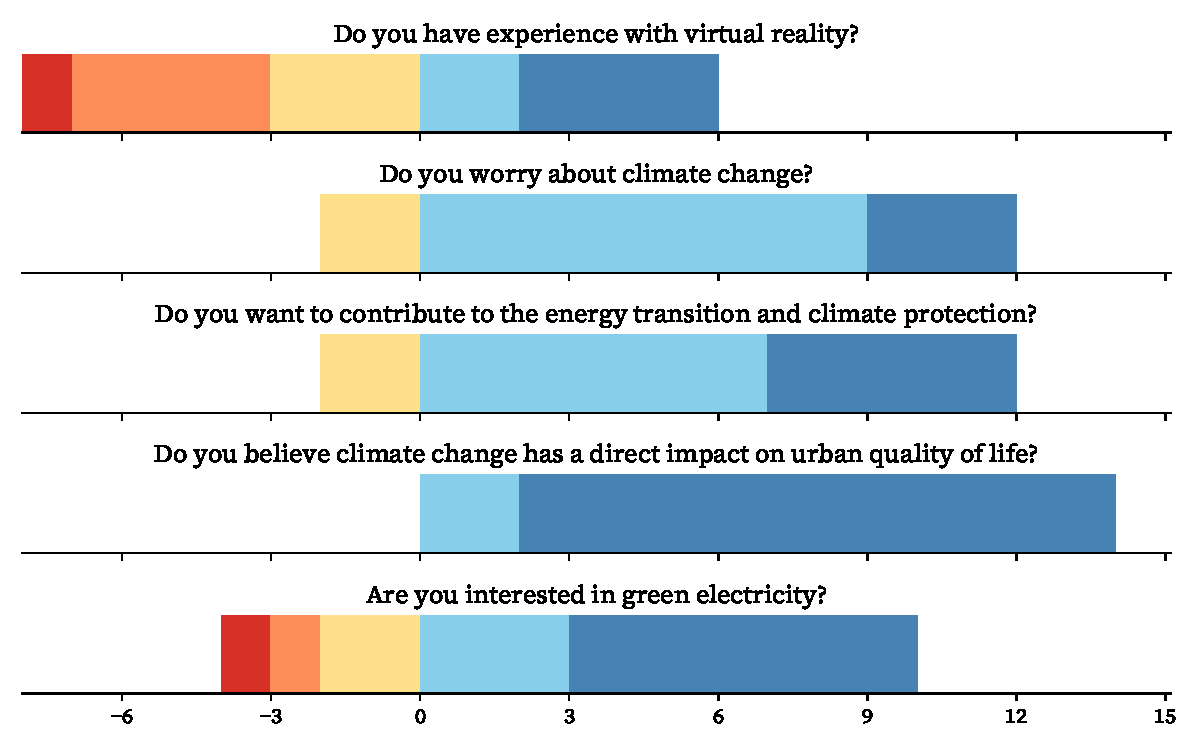
\includegraphics[width=\textwidth]{graphics/participants-kaisergasse.pdf}
    \caption{Stacked bar chart of participant responses to personal questions in the \textit{KaisergasseVR} study. The chart displays answers to questions assessing participants' experience with virtual reality, concerns about climate change, willingness to contribute to energy transition and climate protection, perceptions of climate change's impact on urban quality of life, and interest in green electricity. The color gradient progresses from red (strongly disagree) to blue (strongly agree) on the Likert scale.}
    \label{fig:participants_kaisergasse}
\end{figure}

Participants reported moderate familiarity with VR technologies (mean: 3.286, SD: 1.332), indicating varied experience levels. The participants demonstrated a high level of agreement on the significance of climate change (mean: 4.071, SD: 0.593). They also exhibited a willingness to engage in energy transition activities (mean: 4.214, SD: 0.674), indicating a positive inclination towards environmental action. Furthermore, they expressed a strong belief in the impact of climate change on urban quality of life (mean: 4.857, SD: 0.350). There was a moderate level of interest in eco-electricity (mean: 4.000, SD: 1.254). These responses are visually summarized in \figurename~\ref{fig:participants_kaisergasse}.

\section{User study on \textit{SolarPowerVR}}

The user study on \textit{SolarPowerVR} was conducted during the \textit{VR-Day} event at HLW Steyr. This event was attended by students from one class of HLW Steyr and lasted three hours, from 13:00 to 16:00. The event began with a detailed presentation on the ongoing challenges and achievements in energy transition, including a highlight of our exhibition at Ars Electronica 2023. This served to set the context for the importance of renewable energy solutions, specifically photovoltaic systems. Following the presentation, students had the opportunity to experience \textit{SolarPowerVR} and various VR games. The feedback was overwhelmingly positive.

The setup included four PC-VR stations, each offering a different experience:
\begin{itemize}
    \item Two stations dedicated to \textit{SolarPowerVR}, one equipped with a Meta Quest 3 and the other with a Meta Quest 2.
    \item Interactive experiences with \hyperlink{https://store.steampowered.com/app/517160/Richies_Plank_Experience/}{Richie's Plank Experience} and \hyperlink{https://store.steampowered.com/app/620980/Beat_Saber/}{Beat Saber}, both running on Meta Quest 2.
\end{itemize}

This event marked the first public access to the \textit{SolarPowerVR} app, providing an excellent opportunity for gathering study data and valuable feedback. Participation in trying out VR apps was voluntary, as was completing the post-experience survey. A total of 10 students filled out the form at this event.

Additional sessions were later held at HTL Linz (n=5) and my office (n=3) to collect more data and increase the robustness of our dataset.

\subsection{Study Protocol}

Participants were individually invited and given a presentation on the interactive elements of \textit{SolarPowerVR}. The instructional session covered navigation, photovoltaic layout selection, adjusting the month for simulation, starting/stopping the simulation run, and data interpretation within the VR environment. Individual instructional sessions were chosen to provide personalized guidance and ensure that each participant understood the application's features.

To ensure a smooth and effective instructional session, I prepared a structured schema that began with a 2-minute presentation. This introduction provided users with a clear understanding of how to navigate the app, minimizing the need for additional support. However, I remained available to assist users as needed. To validate and refine this approach, I conducted a pilot test with a single user prior to the main event.

After familiarizing themselves with the setup, participants put on their VR headsets and freely explored the simulation. Upon completion, they were invited to provide their insights and feedback through our user study form.

\subsection{Questionnaire Design}

The questionnaire for this study aimed to assess participants' perceptions of climate change and their experience of the VR simulation. It contained Likert-scale questions (from 1: strongly disagree to 5: strongly agree), multiple-choice questions, and open-ended questions:

\begin{itemize}
    \item \textbf{Demographics and Prior Knowledge}: Initial questions collected demographic data and assessed participants' familiarity with VR technology and their concerns about climate change.
    \item \textbf{Effectiveness of the Simulation}: Participants responded to questions about usability and realism of the VR simulation, its effectiveness in conveying benefits and applications of photovoltaic systems, and their likelihood of engaging in climate-positive actions following their experience.
    \item \textbf{Educational Outcomes}: Specific questions tested understanding of optimal orientation of photovoltaic panels for different seasons, directly measuring educational outcomes from the VR experience.
    \item \textbf{User Experience and Feedback}: Open-ended questions invited comments on what participants liked most and least about their experience as well as suggestions for improvement.
\end{itemize}

\subsection{Data Collection and Analysis}

Data was collected through Google Forms for seamless distribution via QR codes that participants could scan with their mobile devices. Responses were later exported to CSV files for analysis using Python.

\subsection{Participants}
The participant cohort consisted of 18 individuals, primarily young students (mean age: 19.1 years, SD: 5.962). Their familiarity with VR technology was modest (mean: 2.722, SD: 1.283), providing a unique perspective on the educational potential of immersive VR applications such as \textit{SolarPowerVR}. Participants expressed moderate concern about climate change (mean: 3.500, SD: 1.014) and a commendable willingness to engage in activities related to energy transition and climate protection (mean: 3.833, SD: 0.687). The perceived impact of climate change on urban quality of life was particularly high (mean: 4.278, SD: 0.931), while interest in using green electricity was more variable (mean: 3.333, SD: 0.745). These responses are summarized visually in \figurename~\ref{fig:participants_solarpowervr}.

\begin{figure}[h]
    \centering
    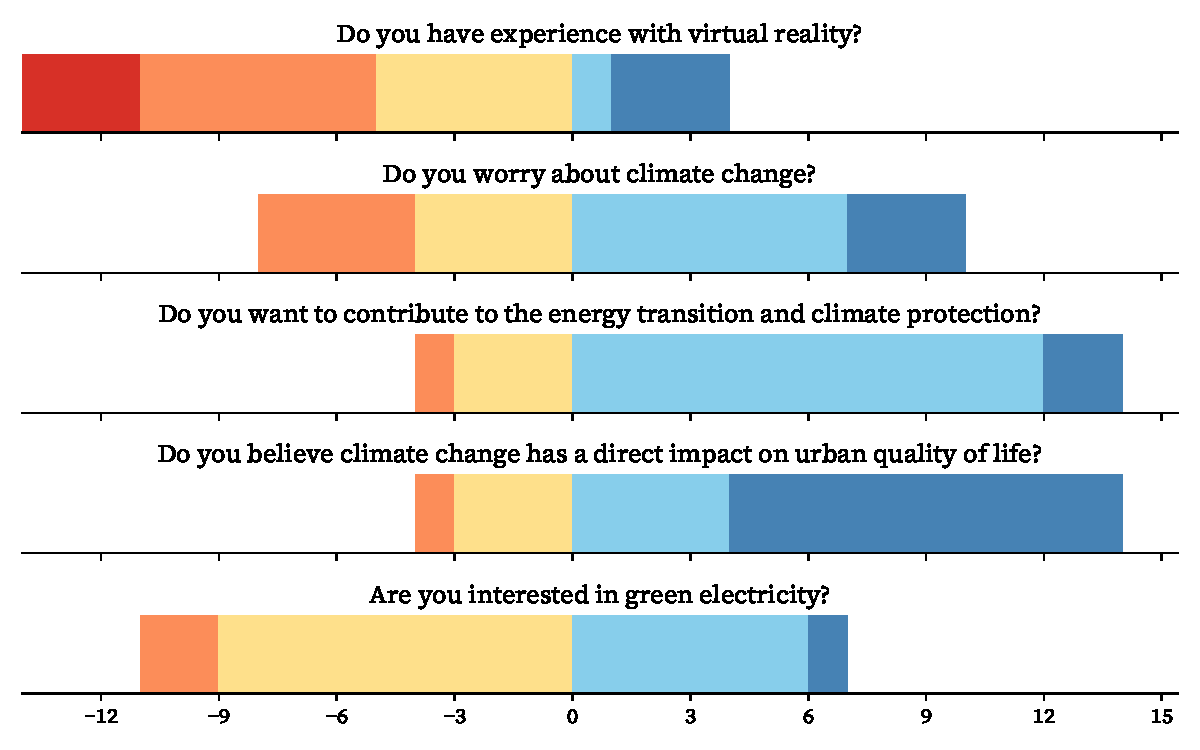
\includegraphics[width=\textwidth]{graphics/participants-solarpowervr.pdf}
    \caption[Participant Responses Summary]{Stacked bar graph showing participants' responses to personal virtual reality experiences, concerns about climate change, engagement in energy transition and climate action, perceived impact on urban quality of life, and interest in green electricity. The color gradient progresses from red (strongly disagree) to blue (strongly agree) on the Likert scale.}
    \label{fig:participants_solarpowervr}
\end{figure}

%nice to have: figure comparing the plots of both user studies

 
\chapter{Results}

This chapter presents the findings of two empirical studies evaluating the efficacy of virtual reality (VR) applications for enhancing public understanding of photovoltaic (PV) systems. The first study examined the existing VR application, \textit{KaisergasseVR}, to establish a baseline understanding of user experience and learning outcomes related to environmental topics. The second study evaluated our newly developed application, \textit{SolarPowerVR}, which focuses specifically on fostering comprehension of PV system principles and benefits, incorporating interactive elements and a focused approach to enhance learning. The results of these studies provide valuable insights into the potential of VR for bridging the gap between technical knowledge and public engagement with sustainable energy technologies.

\section{User Feedback on \textit{KaisergasseVR}} \label{sec:kaisergasse-feedback}

The \textit{KaisergasseVR} application was generally well-received by participants, with high ratings for ease of navigation (mean: 4.000, SD: 0.845). This suggests that the VR environment was perceived as user-friendly and intuitive. The realism of the simulation received a moderately high rating (mean: 3.643, SD: 0.895), indicating a good level of immersion, though there is room for improvement. Participants demonstrated a relatively positive response to the idea of installing a PV system (mean: 3.571, SD: 1.050), suggesting a slight inclination towards actual implementation after experiencing the simulation.  The VR experience also had a moderate impact on inspiring climate action (mean: 3.143, SD: 1.355), indicating some motivation towards environmental involvement. However, the considerable standard deviation suggests that responses regarding climate action were not uniform.
These responses are summarized visually in \figurename~\ref{fig:feedback-kaisergasse}.

\begin{figure}[h]
    \centering
    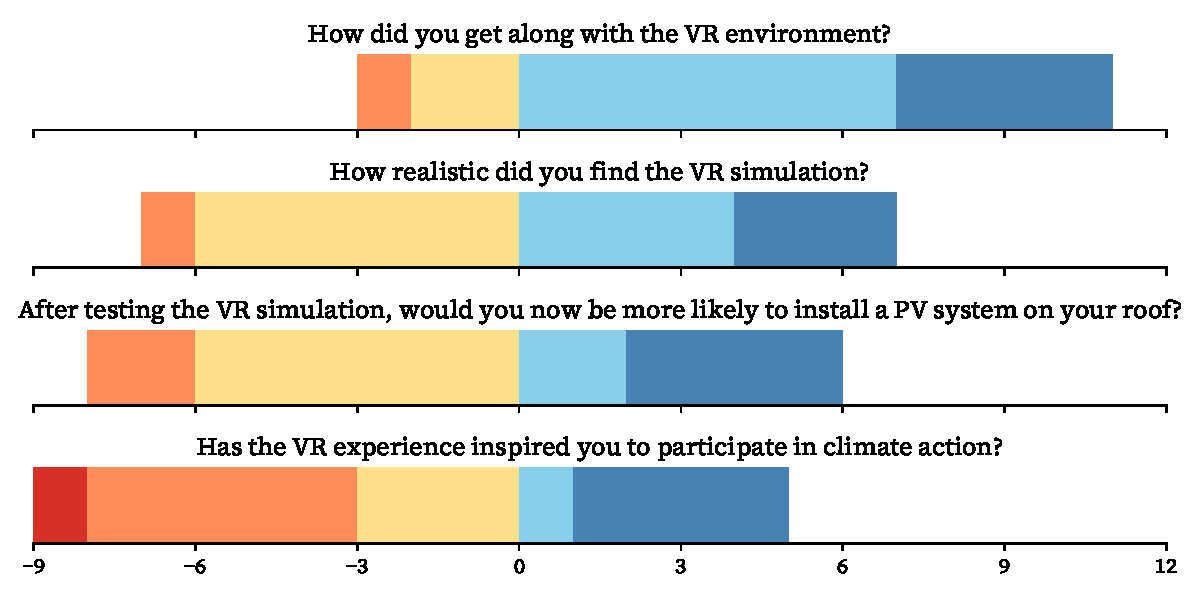
\includegraphics[width=\textwidth]{graphics/feedback-kaisergasse.pdf}
    \caption{Stacked bar chart illustrating the distribution of participant responses to likert scale feedback questions in the \textit{KaisergasseVR} study, including ease of navigation, realism of the simulation, likelihood of installing a PV system, and motivation to engage in climate action. The color gradient progresses from red (strongly disagree) to blue (strongly agree) on the Likert scale.}
    \label{fig:feedback-kaisergasse}
\end{figure}

The participants offered a wealth of insights into the strengths and areas for improvement of the VR application. A synthesis of the responses to the open-ended questions is provided below. 

\subsection{Positive Aspects}

\begin{itemize}
    \item \textbf{Simplicity and Variety of Operations:} Participants appreciated the ease of use and range of options. (e.g., \textit{``The simple execution and various options... were quite nice.''})
    \item \textbf{Effective Use of 360° Photographs:} The integration of real-world imagery enhanced the comparative experience. (e.g., \textit{``The comparison of simulation and the real world''})
    \item \textbf{Tangible Environmental Impact:} Witnessing the visible results of actions like greening increased engagement. (e.g., \textit{``Greening, because the effects are most visibly tangible.''})
    \item \textbf{Immersive Environment and Visuals:} The familiar setting and detailed visuals contributed to a strong sense of immersion. (e.g., \textit{``A very familiar environment... drone recordings were incorporated... variation of the meadow... design of the courtyard''}) 
    \item \textbf{Theme and Relevance:} The content resonated with users, highlighting the importance and appeal of climate-positive actions. (e.g., \textit{``The comparison of simulation and the real world,''} \textit{``Comparison with the real recordings''}) 
\end{itemize}

\subsection{Areas for Improvement and Enhancement Suggestions}

\begin{itemize}
    \item \textbf{Performance and Navigation:} Several participants experienced motion sickness due to inconsistent frame rates, stuttering, and abrupt movements, particularly during flight. (e.g., \textit{``The view shakes a lot,''} \textit{``Motion sickness from flying''})
    \item \textbf{Impact Visualization and Clarity:} Participants desired a clearer understanding of the impact of their actions, particularly regarding features like photovoltaic installations. (e.g., \textit{``Laying photovoltaic panels and power lines didn't really show anything... How quickly was how much energy generated? (e.g., kilometers that you can then drive with the car on average)''})
    \item \textbf{Environmental Enrichment and Detail:} Feedback consistently highlighted the need for a more visually appealing and engaging environment. Suggestions included improved textures, dynamic elements (e.g., animals, people), and decorations to create a more immersive and welcoming atmosphere. (e.g., \textit{``Better textures,''} \textit{``The flower meadow is still missing the buzzing bees :)''} \textit{``Decoration would be great and make the surroundings much friendlier.''})
    \item \textbf{Improved Interaction and Orientation:}  Participants suggested improvements to the interaction mechanics and orientation within the VR environment. This includes smoother rotation, the ability to see virtual hands holding tools, and clearer explanations for certain areas. (e.g., \textit{``The rotation function shouldn't be a sudden jump,''} \textit{``Another idea would be that you can see your own hands in VR''})
    \item \textbf{Solar Panel Feedback:} The proposed feature to simulate energy production based on solar panel orientation was well-received. Participants recommended incorporating visual cues to clearly indicate energy output levels, enhancing the educational aspect of this feature.
\end{itemize}

This user feedback has had a significant impact on the design and development of the \textit{SolarPowerVR} application, addressing previous shortcomings. The new application provides a user-centered experience by focusing on improving \textbf{user comfort}, enriching the \textbf{visual and interactive quality} of the environment, and effectively \textbf{communicating the impact} of climate positive actions.

\section{User Feedback on \textit{SolarPowerVR}}

Participants' interactions within the VR environment were very positive in terms of ease of navigation (mean: 4.389, SD: 0.591).
The realism of the VR simulation received a moderately high rating (mean: 3.778, SD: 0.916), suggesting a convincing yet variable experience across users.
Concerning the potential for action, the simulation influenced participants' willingness to install photovoltaic (PV) systems on their roofs (mean: 3.333, SD: 1.000), indicating a cautious yet positive inclination towards real-world application.
Additionally, the VR experience played a role in inspiring climate action, although to a lesser extent (mean: 3.000, SD: 0.745).
These responses are summarized visually in \figurename~\ref{fig:feedback-solarpowervr}.

\begin{figure}[h]
    \centering
    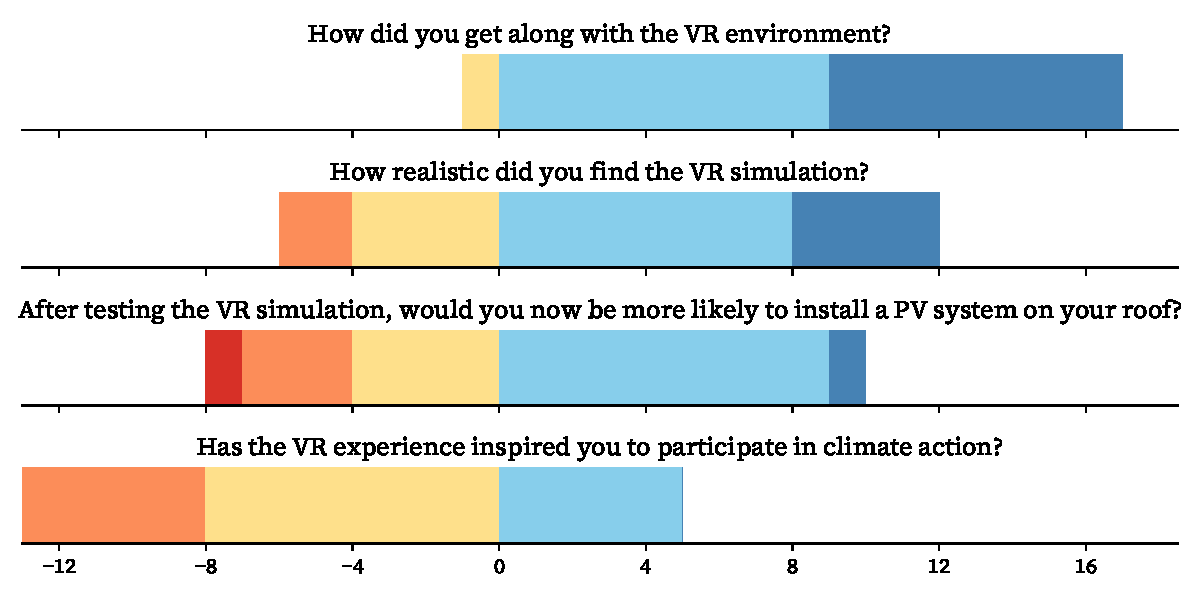
\includegraphics[width=\textwidth]{graphics/feedback-solarpowervr.pdf}
    \caption{Stacked bar chart illustrating the distribution of participant responses to feedback questions in the \textit{SolarPowerVR} study, including ease of navigation, realism of the simulation, likelihood of installing a PV system, and motivation to engage in climate action. The color gradient progresses from red (strongly disagree) to blue (strongly agree) on the Likert scale.}
    \label{fig:feedback-solarpowervr}
\end{figure}

\subsection{Positive Aspects}

\begin{itemize}
    \item \textbf{Interactive Settings and Realistic Representation:} Participants appreciated the ability to adjust settings like the month and time of day and observe their impact on energy calculations. (e.g., \textit{"That you could adjust so many settings (months, time, ...)"}, \textit{"That it was so real"})
    \item \textbf{Hands-on Building and Exploration:} The ability to build structures and navigate the virtual environment was a highlight for many users. (e.g., \textit{"The hands-on building and walking around"})
    \item \textbf{Data Visualization and Energy Calculation:} Users valued the ability to see the number of panels required for specific energy outputs. (e.g., \textit{"You can see how many panels are needed to generate this much energy."})
    \item \textbf{Realistic Visuals and AI Assistant:} The realistic visuals and the helpful AI assistant were praised. (e.g., \textit{"The reality,"} \textit{"Beautiful AI"})
    \item \textbf{Direct Comparison of Setups:} The ability to directly compare different setups and visualize their impact on a rooftop was particularly engaging. (e.g., \textit{"Direct comparison of the different setups and imagining how it would look on the roof."})
\end{itemize}

\subsection{Areas for Improvement and Enhancement Suggestions}

\begin{itemize}
    \item \textbf{AI Assistant Functionality:} Some users reported issues with the AI assistant not functioning correctly. (e.g., \textit{"The AI assistant didn't work unfortunately."})  Improving its reliability and helpfulness is crucial.
    \item \textbf{Limited Activities and Perspective:}  A few participants found the activities within the VR environment limited and expressed a desire for a bird's-eye view of the roof. (e.g., \textit{"You couldn't see the roof from a bird's-eye view."})
    \item \textbf{Environmental Variety and Options:} Suggestions included expanding the virtual environments to include various locations and incorporating additional options like wind turbines. (e.g., \textit{"Different places (cities, park, countries, forests...), other options (wind turbines,...)"})
    \item \textbf{Enhanced Interaction and Guidance:} Participants suggested more activities, step-by-step instructions, and increased interaction with the AI character. (e.g., \textit{"More things to do,"} \textit{"Step-by-step explanations of what to do,"} \textit{"More interaction with the AI person"})
    \item \textbf{Panel Variety and Configuration:} Offering more panel types and configurations could enrich the educational aspect of the simulation. (e.g., \textit{"More versions of the panels"})
\end{itemize}

\section{Impact on Climate Technology Awareness}

This section explores the research question: 

\textbf{Q1: Can a VR simulation like \textit{KaisergasseVR} enhance understanding of and interest in climate-friendly technologies?}

To investigate this, we formulated the following hypotheses:

\textbf{H1: Participants who experience the \textit{KaisergasseVR} simulation will demonstrate a statistically significant increase in their understanding of climate-friendly technologies, specifically green roofs and PV systems.}

\textbf{H2: Participants who experience the \textit{KaisergasseVR} simulation will demonstrate a statistically significant increase in their interest in adopting climate-friendly technologies, specifically green roofs and PV systems.}

To test these hypotheses, we analyzed participant responses to a series of questions related to urban thermal conditions, potential solutions, the benefits of green roofs and PV systems, and their likelihood of adopting these technologies. 

\subsection{Comprehension of Climate-Friendly Solutions}

To assess participants' understanding, we asked the following questions, each rated on a 5-point Likert scale (1 = low understanding, 5 = high understanding):

\begin{itemize}
    \item \textbf{Q1.1} Did the VR experience help you understand urban thermal conditions and potential solutions? (Mean: 3.786, SD: 1.206, Wilcoxon p = 0.02466)
    \item \textbf{Q1.2} Did the VR experience help you understand the benefits of these measures? (Mean: 3.714, SD: 1.221, Wilcoxon p = 0.03301)
\end{itemize}

Scores above the central value of 3 were anticipated to indicate a successful increase in understanding attributable to the VR experience. Analysis of the response distributions using the Shapiro-Wilk test revealed non-normality (p = 0.036 and p = 0.048 for the two questions, respectively), indicating that the data did not meet the assumptions for parametric tests. Therefore, a Wilcoxon signed-rank test, a non-parametric test suitable for small, non-normally distributed samples, was employed to compare the responses to a neutral response of 3 on the Likert scale. This test assesses whether the median of the responses is significantly different from the hypothesized neutral value of 3.

\subsection{Interest in Adopting Green Technologies}

To gauge participant interest in adopting these technologies, we asked:

\begin{itemize}
    \item \textbf{Q1.3} After testing the VR simulation, would you now be more likely to install a green roof? (Mean: 3.714, SD: 1.097, Wilcoxon p = 0.01658)
    \item \textbf{Q1.4} After testing the VR simulation, would you now be more likely to install a PV system on your roof? (Mean: 3.571, SD: 1.050, Wilcoxon p = 0.03097)
\end{itemize}

Again, scores above 3 were anticipated to indicate increased interest. The Shapiro-Wilk test confirmed non-normality in the response distributions for both questions (p = 0.017 for green roofs and p = 0.022 for PV systems), indicating that the data did not meet the assumptions for parametric tests. Therefore, the Wilcoxon signed-rank test was used to compare the responses to a neutral response of 3 on the Likert scale. This non-parametric test is appropriate for analyzing data from a single group when the data is not normally distributed and we want to compare it to a hypothesized median value.

\subsection{Statistical Significance and Interpretation}

While the initial Wilcoxon test results for both understanding and interest suggested a potential positive effect of the VR experience, after applying the Bonferroni correction for multiple testing (α=0.0125, adjusted for 4 tests), the results fell short of statistical significance. The Bonferroni correction was applied to reduce the likelihood of making a Type I error (false positive) when conducting multiple statistical tests.  The results did not support H1, indicating that the \textit{KaisergasseVR} simulation did not lead to a statistically significant increase in participants' understanding of green roofs and PV systems. Similarly, the results did not support H2, suggesting that the simulation did not significantly increase participants' interest in adopting these technologies. While the VR experience may not have resulted in statistically significant changes based on our chosen methodology, the mean scores do suggest a trend towards increased understanding and interest.
Figure~\ref{fig:research-1} provides a visual representation of the participant responses.

\begin{figure}[h]
    \centering
    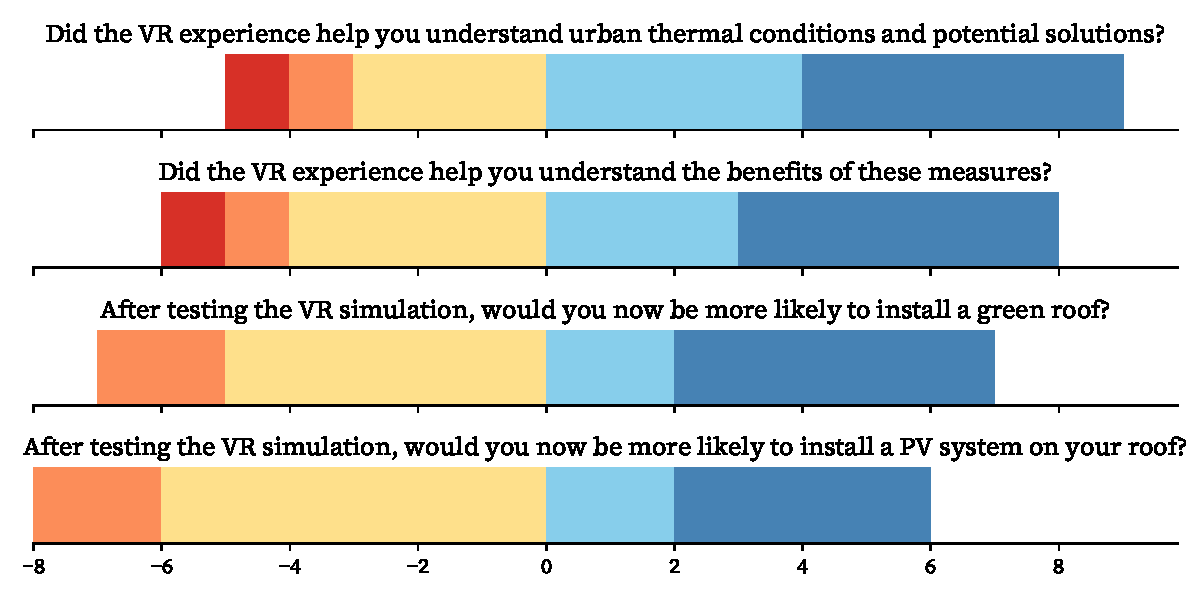
\includegraphics[width=\textwidth]{graphics/research-1.pdf}
    \caption{Participant responses to questions about their comprehension of and interest in climate-friendly technologies, with a focus on urban thermal conditions and solutions, the advantages of green roofs and PV systems, and the probability of adopting these technologies. The color gradient progresses from red (strongly disagree) to blue (strongly agree) on the Likert scale.}
    \label{fig:research-1}
\end{figure}

\section{The Effect of Increased Interactivity on PV Understanding}

This section explores the research question:

\textbf{Q2: Can increased interactive engagement with a photovoltaic (PV) use case in a VR application enhance understanding of and interest in PV solutions?}

To investigate this, we compare participant responses to questions regarding their understanding of PV systems after experiencing two distinct VR applications: \textit{KaisergasseVR} and \textit{SolarPowerVR}. \textit{KaisergasseVR} provides  limited interactivity, while \textit{SolarPowerVR} offers a more interactive environment where users can manipulate PV panel configurations and observe the resulting energy output. This difference in interactivity allows us to assess the impact of interactive engagement on understanding and interest in PV solutions.

We hypothesize:

\textbf{H3: Participants who experience the more interactive \textit{SolarPowerVR} simulation will demonstrate a statistically significant increase in their understanding of and interest in PV solutions compared to those who experience the less interactive \textit{KaisergasseVR} simulation.}

Participants responded to the following questions on a 5-point Likert scale, with 5 being "very helpful" and 1 being "not helpful at all":

\begin{itemize}
    \item \textbf{Q2.1} Did the VR experience help you understand how a photovoltaic system can be used?
    \item \textbf{Q2.2} Did the VR experience help you understand the benefits of a photovoltaic system?
\end{itemize}

\subsection{Analysis and Results}

The data reveals a notable difference in reported understanding between the two VR applications. \textit{KaisergasseVR} demonstrated a lower average understanding (mean: 2.857, SD: 1.245 for use; mean: 3.000, SD: 1.464 for benefits), while \textit{SolarPowerVR} showed a significantly higher average understanding (mean: 4.389, SD: 0.591 for use; mean: 4.278, SD: 0.803 for benefits). Figure~\ref{fig:research-2} visually presents these responses.

The Shapiro-Wilk test indicated non-normality in the distribution of responses for one of the two VR applications in each case, suggesting that the data did not meet the assumptions for a parametric t-test. Therefore, we employed the Mann-Whitney U test, a non-parametric test suitable for comparing two independent groups, to evaluate whether \textit{SolarPowerVR} significantly increased understanding compared to \textit{KaisergasseVR}. This test is appropriate when the data is not normally distributed or when the sample sizes are small. The test was conducted with a one-sided alternative hypothesis, as we anticipated an increase in understanding due to the deliberate focus on interactive elements and information presentation in \textit{SolarPowerVR}. The results revealed significant differences (p = 0.00042 for understanding use, p = 0.00565 for understanding benefits) between the two VR applications, strongly supporting the hypothesis that \textit{SolarPowerVR} led to a greater understanding of PV systems.

\begin{figure}[h]
    \centering
    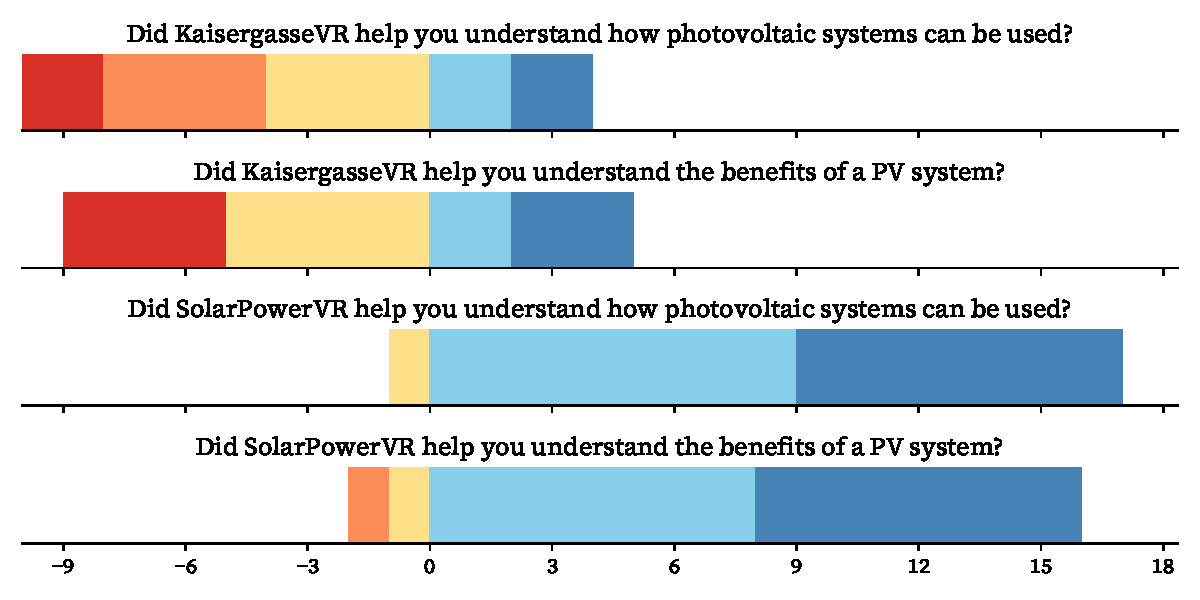
\includegraphics[width=\textwidth]{graphics/research-2.pdf}
    \caption{Stacked bar chart of participant responses on understanding the use and benefits of photovoltaic systems in each application.}
    \label{fig:research-2}
    % reorder the figure items
\end{figure}

This finding provides strong evidence that interactive engagement with a photovoltaic use case in a VR application, particularly one designed with a strong focus on interactive elements and information presentation, significantly increases both understanding of and interest in PV solutions. The ability to manipulate PV panel configurations and observe the resulting energy output in \textit{SolarPowerVR} appears to have contributed to a more profound understanding of PV systems compared to the experience offered by \textit{KaisergasseVR}.

This highlights the importance of incorporating interactive elements and clear information presentation in VR applications designed for educational purposes, especially when aiming to promote understanding and adoption of complex technologies like photovoltaic systems.

\section{Impact of SolarPowerVR on Understanding Panel Orientation}

This section explores the research question:

\textbf{Q3: How effective is an interactive VR simulation in increasing factual knowledge about the optimal orientation of photovoltaic panels?}

To investigate this, we analyze participant responses to questions regarding optimal panel orientation after experiencing the interactive \textit{SolarPowerVR} simulation. We hypothesize that the ability to manipulate panel configurations and observe the resulting energy output in different months within the simulation will lead to a better understanding of optimal orientation.

We hypothesize:

\textbf{H4: Participants who experience \textit{SolarPowerVR} will demonstrate a greater understanding of optimal PV panel orientation than expected by chance.}

A post-experience questionnaire assessed participants' knowledge regarding optimal panel orientation in June, December, and throughout the year. Answer choices included "flat", "inclined south" and "inclined east/west". Correct answers were determined based on the simulation data, implying that mindful observation during the VR experience could lead to correct responses. The questions were designed to be challenging, assuming limited prior knowledge on this topic. We hypothesize that participants who actively engage with the simulation and observe the changes in energy output based on panel orientation will be more likely to answer these questions correctly.

\subsection{Analysis and Results}

The Chi-square test was selected for its suitability in analyzing categorical data (optimal panel orientation) and its ability to compare observed response distributions with those expected by chance. This test is appropriate for evaluating the educational impact of the VR simulation on factual knowledge because it assesses the independence of participant responses and is effective with smaller sample sizes. The Chi-square test determines whether there is a statistically significant association between the observed frequencies and the expected frequencies based on chance. A small p-value (p < α) indicates that the observed data is unlikely to have occurred by chance alone, leading us to reject the null hypothesis and conclude that the VR simulation likely had an effect on participants' understanding of optimal panel orientation.
Figure~\ref{fig:research-3} visually presents the distribution of participant responses. Table~\ref{tab:chi-square-results} summarizes the Chi-square test results for each question.

\begin{table}[h]
    \centering
    \begin{tabular}{llll}
    \toprule
    \textbf{Orientation} & \textbf{Correct Responses} & \textbf{Chi-square Test} & \textbf{Result} \\
    \midrule
    June & 38.9\% (7 out of 18) & χ² = 2.333, p = 0.311 & Supports $H_0$ \\
    December & 55.6\% (10 out of 18) & χ² = 4.000, p = 0.135 & Supports $H_0$ \\
    Annual & 44.4\% (8 out of 18) & χ² = 1.333, p = 0.513 & Supports $H_0$ \\
    \bottomrule
    \end{tabular}
    \caption{Chi-square Test Results for Optimal PV Panel Orientation}
    \label{tab:chi-square-results}
\end{table}

\begin{figure}[]
    \centering
    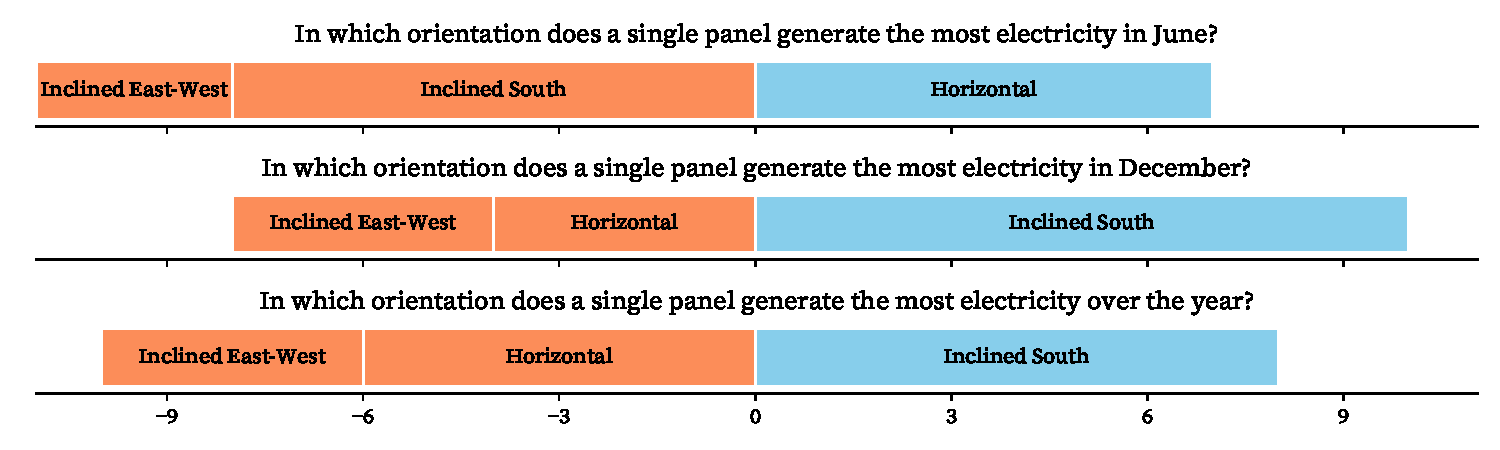
\includegraphics[width=\textwidth]{graphics/research-3.pdf}
    \caption{Distribution of participant responses regarding optimal photovoltaic panel orientation for electricity production in June, December, and throughout the year. Blue bars represent correct answers, and orange bars represent incorrect answers.}
    \label{fig:research-3}
\end{figure}

While the observed percentages of correct answers for December and annual orientation are above chance (33.3\%), the Chi-square tests indicate that these deviations are not statistically significant. This suggests that the \textit{SolarPowerVR} simulation, as designed, did not significantly improve factual knowledge about optimal PV panel orientation. However, the higher percentages of correct responses compared to random chance warrant further investigation and suggest potential avenues for improving the educational effectiveness of the simulation.


\chapter{Discussion}

This chapter delves into the implications of the research findings, exploring the potential of virtual reality (VR) as an educational tool for promoting understanding and engagement with photovoltaic systems. We examine the strengths and limitations of the VR applications, \textit{KaisergasseVR} and \textit{SolarPowerVR}, highlighting the insights gained from the statistical analysis of learning outcomes. We will address each research question individually, discussing the findings and their implications for the design and implementation of VR educational experiences.

\section{Impact on Climate Technology Awareness}

Our first research question explored whether a VR simulation like *KaisergasseVR* could enhance understanding of and interest in climate-friendly technologies. While the statistical analysis did not reveal a significant impact, the observed trend towards increased understanding and interest, coupled with participant feedback, warrants further discussion.

The mean scores for both understanding and interest in adopting climate-friendly technologies were above the neutral point on the Likert scale. This suggests that the VR experience may have had a positive, albeit not statistically significant, influence. While \textit{KaisergasseVR} lacks some interactivity and best practices from established scientific literature \cite{Dalgarno2010Learning, Gee2009Deep}, which limits its potential, the immersive nature of VR could still have contributed to this positive trend. It's important to note that \textit{KaisergasseVR} lacked any interactivity with the PV system beyond a one-click installation, and feedback was limited to displaying green cables. This suggests that while participants may have been made aware of PV technology, they did not have the opportunity to learn about its functionality or benefits in detail.

However, participant feedback sheds light on potential reasons for the lack of statistical significance. Several participants noted a lack of clarity regarding the impact of their actions within the simulation, particularly with the PV system. This suggests that the simulation may not have effectively conveyed the connection between user actions and their environmental consequences, hindering a deeper understanding of the technologies presented.

This feedback aligns with research highlighting the importance of clear cause-and-effect relationships in VR learning experiences \cite{Bailenson2008Transformations, Merchant2014VrEffectiveness}. When users can clearly see the impact of their actions within the virtual environment, they are more likely to develop a deeper understanding of the underlying concepts. This reinforces the need for careful design choices that effectively communicate the connection between user actions and their real-world consequences \cite{Ding2022VrApplication}.

\section{The Effect of Increased Interactivity on PV Understanding}

Our second research question investigated whether increased interactive engagement with a photovoltaic (PV) use case in a VR application could enhance understanding of and interest in PV solutions. To address this, we compared participant responses after experiencing two distinct VR applications: \textit{KaisergasseVR}, which offers limited interactivity, and the more interactive and focused \textit{SolarPowerVR}.

While \textit{KaisergasseVR} demonstrated the potential of VR for raising awareness, the study highlighted the need for more interactive and engaging experiences to foster a deeper understanding of specific technologies like photovoltaic systems. This led to the development of \textit{SolarPowerVR}, which was designed to specifically target PV systems, incorporating various VR best practices to promote learning and engagement \cite{Dalgarno2010Learning, Gee2009Deep}. These design elements, discussed in detail in the Approach chapter, aimed to create a more impactful and engaging learning experience. It allows users to manipulate PV panel configurations, observe the resulting energy output in different months, and explore the impact of various factors, such as the sun's position, on PV system performance.

The results clearly demonstrated a significant difference in reported understanding between the two applications. Participants who experienced \textit{SolarPowerVR} showed a significantly higher average understanding of both how a photovoltaic system can be used and the benefits of such systems. This finding strongly supports the hypothesis that increased interactivity and a focused approach can lead to a more profound understanding of PV solutions.

This is further supported by participant feedback. Many praised the ability to manipulate PV panel configurations and observe the resulting energy output, highlighting the value of hands-on experimentation in fostering a deeper understanding of PV systems. This aligns with research showing that embodied learning experiences in VR, where users can actively interact with virtual objects and environments, can lead to improved learning outcomes \cite{Sung2015Effects, Winn2002Immersion}.

This finding also aligns with the principles of constructivist learning theory \cite{Mikropoulos2011VrEducational}. By providing users with the opportunity to actively engage with the subject matter and explore its nuances, VR can facilitate a more profound and lasting understanding of complex concepts like photovoltaic systems. The design of \textit{SolarPowerVR}, with its emphasis on user agency, accurate simulation, and clear data visualization, exemplifies these principles and demonstrates their effectiveness in enhancing learning outcomes.

The significantly higher understanding demonstrated by participants who experienced \textit{SolarPowerVR} underscores the potential of well-designed, interactive VR experiences to enhance learning outcomes in environmental education. By providing users with the opportunity to actively engage with the subject matter and explore its nuances, VR can facilitate a more profound and lasting understanding of complex concepts.

\section{Impact of SolarPowerVR on Understanding Panel Orientation}

Our third research question explored the effectiveness of an interactive VR simulation in increasing factual knowledge about the optimal orientation of photovoltaic panels. Specifically, we investigated whether experiencing \textit{SolarPowerVR} would lead to a greater understanding of optimal panel orientation for maximizing electricity production. The findings regarding the effectiveness of interactive engagement in \textit{SolarPowerVR} raise questions about whether this approach also translates to the acquisition of specific factual knowledge. To investigate this, we examined participants' understanding of optimal PV panel orientation.

The results of the Chi-square tests, however, did not support this hypothesis. While the observed percentages of correct answers for December and annual orientation were above chance, these deviations were not statistically significant. This suggests that \textit{SolarPowerVR}, as designed, did not significantly improve factual knowledge about optimal PV panel orientation.

This finding aligns with feedback from participants who expressed a desire for more explicit guidance and explanations within the simulation. Some participants noted that while they enjoyed experimenting with the panel configurations, they felt unsure about the optimal orientation for maximizing energy output. This suggests that the simulation, while effective in promoting exploration and engagement, may have lacked the necessary scaffolding to facilitate the acquisition of specific factual knowledge. This aligns with research highlighting the importance of scaffolding and explicit instruction in VR learning experiences, particularly for complex concepts \cite{Dalgarno2010Learning, Mikropoulos2011VrEducational}. Providing explicit guidance on optimal panel orientation, could enhance the educational effectiveness of the simulation in future iterations.

The lack of statistically significant improvement in factual knowledge highlights the importance of considering the specific learning objectives when designing VR educational experiences. While interactivity and exploration can be valuable for promoting engagement and conceptual understanding, they may not be sufficient for acquiring factual knowledge, especially when dealing with complex topics like optimal PV panel orientation. For instance, studies have shown that incorporating explicit instruction and guidance within VR simulations can significantly improve learning outcomes related to factual knowledge acquisition \cite{Merchant2014VrEffectiveness}.

Despite the lack of statistically significant improvement, the higher percentages of correct responses compared to random chance suggest that \textit{SolarPowerVR} may still have had a positive influence on participants' understanding of optimal PV panel orientation. This, combined with the participant feedback, suggests that future iterations of the application could benefit from incorporating more explicit instruction, visual cues, or interactive tutorials that directly address the concept of optimal orientation.

\section{Strengths and Limitations}

This study explored the potential of virtual reality (VR) as an educational tool for promoting understanding and engagement with photovoltaic systems. The use of immersive VR technology allowed participants to experience and interact with PV systems in a way that would otherwise not be possible. This immersive and interactive approach is a key strength of the study, offering a unique and engaging learning experience that can enhance understanding and motivation. VR's ability to create a sense of presence and engagement \cite{Winn2002Immersion, HuAu2018VrExperience} allows users to connect with the subject matter on a deeper level, potentially fostering a more profound understanding and a greater appreciation for the complexities of photovoltaic systems.

However, the study also has several limitations that should be acknowledged:

\begin{itemize}
    \item \textbf{Potential for Benchmark Overfitting:} The design of \textit{SolarPowerVR} specifically addressed the limitations of \textit{KaisergasseVR}, potentially leading to an overfitting of the benchmark and inflating the observed differences between the two applications. This tailored design, while insightful, may limit the generalizability of the findings.
    \item \textbf{Small Sample Size:} The limited number of participants (n=18) may have restricted the statistical power of the analyses and the generalizability of the findings. This sample size, while common in exploratory VR studies, could have made it more difficult to detect statistically significant effects. 
    \item \textbf{Lack of Pre-Test:} The absence of a pre-test measuring baseline understanding and interest makes it difficult to definitively attribute any observed changes to the VR experience. Without a baseline measurement, it's challenging to isolate the specific impact of the VR intervention. 
    \item \textbf{Choice of Likert Scale:} The 5-point Likert scale may have limited the sensitivity of the measurements and made it challenging to apply certain statistical tests. A wider scale might have provided more nuanced data, potentially allowing for more sophisticated statistical analysis. 
    \item \textbf{Lack of Long-Term Knowledge Retention Assessment:} The study did not assess the long-term retention of knowledge gained through the VR experiences. The long-term impact of the VR interventions on knowledge retention remains an open question.
    \item \textbf{Ethical Considerations:} the study had limitations regarding data anonymization and retention. Participant data was not fully anonymized, and a specific data retention period was not defined. This raises potential concerns about participant privacy and confidentiality, highlighting the need for more robust anonymization procedures and clear data retention policies in future research.
\end{itemize}

Despite these limitations, the study provides valuable insights into the potential of VR as an educational tool for promoting understanding and engagement with photovoltaic systems. The findings suggest that VR experiences can be effective in enhancing understanding, particularly when they incorporate interactive elements and a focused approach.

\section{Implications}

This section synthesizes the insights gained from participant feedback and discusses the broader implications of the study's findings, not only for VR in environmental education but also for related fields.

Participant feedback highlighted the need for intuitive navigation and user interfaces, emphasizing the importance of user-centered design principles in VR applications. This reinforces the need for significant technical expertise and careful attention to user experience design when developing immersive and effective VR applications. Performance optimization, especially for resource-intensive environments, is critical to ensure a smooth and engaging user experience, while delivering aesthetically pleasing visuals. The design of VR applications should be driven by user feedback, iteratively refining interfaces, controls, and content based on user needs and preferences.

The findings and feedback from this study suggest that VR holds significant potential not only for environmental education but also for broader scientific communication and public engagement with complex scientific topics. The insights gained can be applied to other domains where VR could enhance understanding and engagement. Key design considerations for creating effective learning experiences across various scientific disciplines include incorporating clear feedback mechanisms, interactive elements, immersive environments, and user-friendly design. These principles can be applied to the development of various interactive learning experiences, even those that do not involve VR technology.

This study's findings connect to the broader fields of computer simulation and visualization, highlighting the potential to make complex scientific data more accessible and engaging. Developing accessible simulations that cater to diverse learning styles and abilities is crucial for reaching a wider audience, including individuals with disabilities or limited access to technology. The insights gained can contribute to the advancement of training and education in fields where hands-on experience are particularly valuable.

This study has demonstrated the potential of VR to enhance understanding and engagement with photovoltaic systems, offering valuable insights for designing more effective VR learning experiences in environmental education and beyond. Further exploration in these areas will contribute to a deeper understanding of how VR can be leveraged to address pressing environmental challenges and promote a more sustainable future.

\chapter{Conclusion and Future Work}

This thesis has demonstrated the feasibility and potential of VR as a powerful tool for promoting understanding and engagement with sustainable energy solutions, particularly focusing on PV systems. Through the development and evaluation of \textit{SolarPowerVR}, a novel VR application specifically tailored to enhance understanding of PV systems, we have gained valuable insights into the potential and limitations of VR for environmental education. Our research has shown that interactive engagement in VR-based learning can significantly enhance user understanding of PV systems compared to less interactive experiences. However, we also discovered that interactivity alone may not be sufficient for acquiring specific factual knowledge, such as optimal panel orientation, highlighting the importance of balancing interactivity with clear instruction and guidance in VR educational applications. 

Our research has yielded several key findings and contributions:

\begin{itemize}
    \item \textit{SolarPowerVR}, with its interactive design, significantly increased participants' understanding of PV system functionality and benefits compared to the less interactive \textit{KaisergasseVR}.
    \item While \textit{SolarPowerVR} promoted engagement and exploration, it did not significantly improve factual knowledge about optimal PV panel orientation, suggesting the need for more explicit instruction and guidance.
    \item The immersive and interactive nature of VR can make complex scientific concepts more tangible and relatable, offering potential for broader applications in scientific communication and public engagement.
\end{itemize}

\section{Future Research Directions}

Building upon the foundation laid by this thesis, we identify promising avenues for future research that focus on enhancing user engagement and learning through interactive design. Future research could explore the effectiveness of incorporating diverse VR interaction modalities, such as hand tracking and haptic feedback, in conjunction with well-designed instructional elements to create a more engaging and intuitive learning experience. This could involve investigating how allowing users to physically manipulate virtual PV panels with their hands or experience the sensation of connecting wires, combined with clear explanations and visual cues, can improve learning outcomes and foster a deeper understanding of PV system dynamics.

\section{Development Plans: Expanding the Simulation}

Future development of \textit{SolarPowerVR} will focus on expanding the scope and realism of the simulation while enhancing its educational value and user experience, incorporating insights from our research and user feedback.  We aim to enhance the realism and immersiveness of the virtual environment by utilizing photogrammetry to create a highly detailed and realistic 3D model of the immediate environment. We also plan to incorporate features such as energy storage options, electric vehicle charging, dynamic cloud cover, and realistic panel shadowing to provide a more comprehensive and realistic simulation of PV system integration and benefits. This expanded scope will allow users to explore a wider range of scenarios and gain a deeper understanding of the complexities of PV systems in real-world contexts. 

Additionally, we plan to enhance the AI assistant to provide real-time, context-aware instruction, personalized guidance, and adaptive feedback based on user actions and progress. This will involve developing a deeply integrated AI character capable of understanding user needs, providing tailored support throughout the learning experience, and acting within the environment. 

To ensure greater accessibility and inclusivity, we will expand language support and optimize \textit{SolarPowerVR} for lower-end hardware. This will broaden the application's reach and make it available to a wider range of users, including those with limited access to high-performance VR equipment.

\section{Broader Impact and Potential Applications}

The insights gained from this research have implications beyond environmental education, offering valuable lessons for the design of effective VR learning experiences across various scientific disciplines. 

\textit{SolarPowerVR} has already reached a diverse range of stakeholders, including students, educators, policymakers, and the general public, through its incorporation into workshops conducted by Verein Energiewende Linz, presentations to the Bildungsministerium, and showcases at \href{https://kinderuni.at/kinderuniwien/infos-und-termine/}{Kinderuni 2024} and \href{https://ars.electronica.art/hope/de/}{Ars Electronica 2024}. We are actively seeking partnerships with educational institutions to make \textit{SolarPowerVR} more widely available and accessible. We believe that \textit{SolarPowerVR} has the potential to inspire and inform discussions about renewable energy adoption and climate action, contributing to a more sustainable future for Austria and beyond. We are hopeful that future funding and partnerships will support further development and wider application of \textit{SolarPowerVR}, allowing us to realize its full potential for promoting sustainable energy solutions.

\section{Reflection on the Research Process}

Developing the VR applications and conducting the user studies was a deeply enriching experience, albeit a challenging one. 

The steepest learning curve for me was mastering the diverse range of new technologies required for this project. Coming from a web development background with experience in UI/UX, I had to quickly learn Unreal Engine, C++, 3D modeling, performance optimization techniques, and the intricacies of VR development. This rapid learning process, coupled with the demands of precise simulation and statistical analysis, pushed me beyond my comfort zone.

Personally, managing the demands of this research alongside my other responsibilities presented significant challenges. The intense focus required for developing the application and writing the thesis, combined with the time constraints and limited resources, led to periods of intense pressure and significant strain. This experience has provided me with valuable insights into the importance of maintaining a healthy work-life balance, especially when undertaking ambitious research projects.

Throughout this journey, I received invaluable support from my advisor Katharina Krösl, and the team at Energiewende Linz. Their guidance, expertise, and collaborative spirit were essential to the success of this project. I am deeply grateful for their contributions and unwavering support.

The challenges I faced and the insights I gained have fueled my passion for developing impactful VR applications that promote sustainable energy solutions. I am committed to continuing this work and exploring the full potential of VR to revolutionize environmental education and empower individuals to make informed decisions about their energy choices.

\backmatter

% Use an optional list of figures.
\listoffigures % Starred version, i.e., \listoffigures*, removes the toc entry.

% Use an optional list of tables.
% \cleardoublepage % Start list of tables on the next empty right hand page.
% \listoftables % Starred version, i.e., \listoftables*, removes the toc entry.

% Use an optional list of alogrithms.
% \listofalgorithms
% \addcontentsline{toc}{chapter}{List of Algorithms}

% Add an index.
\printindex

% Add a glossary.
\printglossaries

% Add a bibliography.
\bibliographystyle{ieeetr}
% \bibliographystyle{plain}
% \bibliographystyle{alpha}
\bibliography{main}

\end{document}
